% TODO: Check lines for listings! They have changed.

\chapter{Expert Questionnaire}\label{chapter: expert}

    % Inhalt des Kapitels, Ziel, (Grund für Befragung)
    %
    %  (-> Validierte Liste von SDKs im Space, Meinungen zu den Lösungen, Was ist (nicht)       wichtig, Kriterien? ...)
    
    After the theoretical foundations have been laid out in the last chapter, this chapter prepares the subsequent work on the reference implementation and the evaluation framework. For this purpose, a questionnaire of experts in the \ac{SSI} space is prepared in the following sections and its conduction and results are documented. This will provide the technical and factual basis for the further procedure. In the next section, the preparation of the survey will be presented first.
   
    \section{Preparation}
    % Herangehensweise: Recherche + Community Meetings -> IIW April
    %
    %  Recherche: Übersicht über generelle Projekte -> Filtern von SDKs & Co.
    %  -> Tabelle mit wichtigsten SDKs im SSI Space 
    % 
    %  IIW: Gefühl für aktuelle Bemühungen, Projekte, Personen
    %  -> Liste: Experten, vorgeführte SDKs
    % 
    % Fragen definieren: Was will ich erreichen? Welche Fragen notwendig? Umfang?
    
    The survey of experts in the field is intended to ensure that the work and its artefacts are based on practical experience and opinions. On the one hand, the goal is to confirm the importance of the Developer Experience (DX), but also to generate a validated list of \ac{SSI} solutions. In addition, it is to be determined which of the solutions are recommendable or not, which criteria are relevant for the selection and which aspects are currently possibly still underrepresented in the solutions.
    
    % integrate citations (ssi tabelle)
    Starting with the list, a literature \cite{bouras_distributed_2020, bernabe_privacy-preserving_2019, dib_decentralized_2020, dunphy_first_2018, ferdous_search_2019, kuperberg_blockchain-based_2020, van_bokkem_self-sovereign_2019, friedewald_self-sovereign_2020,gruner_relevance_2018}, and internet search was first conducted to create an initial and rough overview of existing solutions. This proved to be a complicated undertaking, as the literature often discusses old (uPort) or SDK-less solutions (ShoCard) and sometimes even mixes in \ac{SSI} networks. For example, Sovrin as a Hyperledger network was often found in the same table as uPort \cite{bouras_distributed_2020, bernabe_privacy-preserving_2019, dib_decentralized_2020, dunphy_first_2018}. This is confusing and not helpful for the respective developers who want to integrate \ac{SSI} into their products. Therefore, solutions were first filtered out that are also correspondingly open for developers. Afterwards, it was checked which steps of the \ac{vc} lifecycle \cite{sporny_verifiable_2019} the individual solutions can cover. This is relevant for checking the extent to which the solutions could meet implementation requirements. For this purpose, the websites, and documentations of the individual solutions were checked, which unfortunately often contain only little information.
    
    To extend the table even further, some talks at the \ac{IIW} in April 2021 were followed, from which Mattr, Trinsic, and Veramo could be added. Those solutions are backed by experts who also contribute to various standards in the \ac{SSI} space and are thus among the most important solutions. Nevertheless, there is still little mentioning of them in the analysed literature. These observations resulted in table \ref{tab: draft overview}, which shows the name of the found solutions, the type, and the coverage of the \ac{vc} lifecycles. It is important to mention that the contents of this table are partly based on vague information and should therefore be treated with caution. Therefore, a validation by experts and a practical test of the most important solutions in the context of a reference implementation is essential to generate reliable data.

    \begin{table}[htp]
        \centering
        \caption{Initial solution overview}
        \begin{tabular*}{\textwidth}{l @{\extracolsep{\fill}} llllllllll}
        \toprule \vspace{1.5em} \\
        \textbf{Name} & \textbf{Type} & \begin{rotate}{45}\textbf{Issue}\end{rotate} & \begin{rotate}{45}\textbf{Store}\end{rotate} & \begin{rotate}{45}\textbf{Transfer}\end{rotate} & \begin{rotate}{45}\textbf{Compose}\end{rotate} & \begin{rotate}{45}\textbf{Present}\end{rotate} & \begin{rotate}{45}\textbf{Verify}\end{rotate} & \begin{rotate}{45}\textbf{Revoke}\end{rotate} & \begin{rotate}{45}\textbf{Delete}\end{rotate}  \\ 
        \midrule
        Mattr                              & Platform                           & \ding{51}                              & \ding{55}                               & \ding{55}                                   & \ding{51}                                & \ding{51}                                & \ding{51}                               & \ding{51}                               & \ding{51}                                \\
        vc-js (Digital Bazaar)             & Library                            & \ding{51}                              & \ding{55}                                & \ding{55}                                   & \ding{51}                                & \ding{55}                                  & \ding{51}                               & \ding{55}                                 & \ding{55}                                  \\
        Azure AD for VCs                   & Platform                           & \ding{51}                              & \ding{51}                              & \ding{55}                                   & \ding{51}                                & \ding{51}                                & \ding{51}                               & \ding{51}                               & \ding{51}                                \\
        Evernym                            & SDK                                & \ding{51}                              & \ding{51}                              & \ding{55}                                   & \ding{51}                                & \ding{51}                                & \ding{51}                               & \ding{51}                               & \ding{51}                                \\
        \vcell{Veramo}                     & \vcell{Framework}                  & \vcell{\ding{51}}                      & \vcell{\ding{55}}                        & \vcell{\ding{55}}                           & \vcell{\ding{51}}                        & \vcell{\ding{55}}                          & \vcell{\ding{51}}                       & \vcell{\ding{55}}                         & \vcell{\ding{55}}                          \\[-\rowheight]
        \printcellbottom                   & \printcellbottom                   & \printcellbottom                    & \printcellbottom                    & \printcellbottom                       & \printcellmiddle                      & \printcellmiddle                      & \printcellmiddle                     & \printcellmiddle                     & \printcellmiddle                      \\
        Identity.com (Connect.me)                     & Library                            & \ding{51}                              & \ding{51}                              & \ding{55}                                   & \ding{55}                                  & \ding{51}                                & \ding{51}                               & \ding{55}                                 & \ding{55}                                  \\
        Jolocom                            & Library, SDK                       & \ding{51}                              & \ding{51}                              & \ding{55}                                   & \ding{55}                                  & \ding{51}                                & \ding{51}                               & \ding{55}                                 & \ding{55}                                  \\
        Trinsic                            & Platform                           & \ding{51}                              & \ding{51}                              & \ding{55}                                   & \ding{51}                                & \ding{51}                                & \ding{51}                               & \ding{51}                               & \ding{51}                                \\
        Dock                               & SDK                                & \ding{51}                              & \ding{55}                                & \ding{55}                                   & \ding{51}                                & \ding{55}                                  & \ding{51}                               & \ding{51}                               & \ding{55}                                  \\
        vc.js (Transmute)                  & Library                            & \ding{51}                              & \ding{55}                                & \ding{55}                                   & \ding{51}                                & \ding{55}                                  & \ding{51}                               & \ding{55}                                 & \ding{55}                                  \\
        TangleID                           & Library                            & \ding{51}                              & \ding{55}                                & \ding{55}                                   & \ding{55}                                  & \ding{55}                                  & \ding{51}                               & \ding{55}                                 & \ding{55}                                  \\
        Affinidi                           & Platform                           & \ding{51}                              & \ding{51}                              & \ding{55}                                   & \ding{51}                                & \ding{51}                                & \ding{51}                               & \ding{51}                               & \ding{51}                                \\
        DIDKit                             & Library                            & \ding{51}                              & \ding{55}                                & \ding{55}                                   & \ding{51}                                & \ding{55}                                  & \ding{51}                               & \ding{55}                                 & \ding{55}
        \tabularnewline
        \bottomrule
        \end{tabular*}
        \label{tab: draft overview}
    \end{table}
    
    In addition, this table has a rather illustrative value, not a comprehensive one, since this work is not meant to cover all existing solutions on the market but merely provides a rough overview of notable and important projects. Looking at the lifecycle, it becomes clear that the solutions differ greatly in their range of functionality, which is particularly noticeable with regard to their types. Thus, libraries usually focus on individual areas, while platforms, frameworks, and SDKs often cover larger areas. In addition, the store step only refers to the presence of a wallet, which is why solutions such as Veramo did not receive a check here despite the presence of agent-internal storage. 
    
    Now that an initial overview has been created, the definition of the questions will be addressed at this point. The questions follow the basic subjects defined at the beginning of the section. In addition, a manageable number of questions as broad as possible were chosen to make the answering process as convenient as possible and thus to incentivize it. This resulted in the following questions:
    
    \begin{enumerate}
        \item What is your job title? (Developer, Researcher, ...)		
        \item Are you currently working on  anything SSI-related?		
        \item What fascinates you about SSI?		
        \item What value would you attribute to the experience of a developer concerning its available toolset for the successful implementation of SSI products?		
        \item Looking at the spreadsheet, what additions or changes would you make?		
        \item If you were a developer at a company looking to integrate Verifiable Credentials into their products, which three solutions would you look at and why?		
        \item Which ones wouldn't you use and why?		
        \item What do you consider essential criteria for selecting a good SSI solution for implementing Verifiable Credentials?		
        \item What do you think are common problems existing SSI solutions for developers have? 
        \item Is there something you still want to say?
    \end{enumerate}
    
    Regarding the selection of experts, the participation in the \ac{IIW} in April 2021 was very helpful, as a large part of the SSI community attended. On the one hand, technical talks and their subsequent discussions were followed in order to identify experts with technical expertise. From this and own internet research, table X was created, which summarizes the names, companies and positions of the individual experts.

    \begin{table}[htp!]
        \centering
        \caption{Expert list}
        \begin{tabular*}{\textwidth}{l @{\extracolsep{\fill}} lll}
        \toprule
        \textbf{Name}      & \textbf{Company}                & \textbf{Position}                                   \\ \midrule
        Adolf, Stefan      & Turbine Kreuzberg               & Developer Ambassador                                \\
        Buchner, Daniel    & Microsoft                       & Senior PM - Decentralized Identity                  \\
        Curran, Stephen    & Cloudcompass                    & Technical Architect                                 \\ 
        Den Hartog, Kyle   & MATTR                           & Senior Standards Engineer                           \\
        Du Seuil, Daniël   & \begin{tabular}[t]{@{}l@{}}European \\ Blockchain Partnership\end{tabular} & \begin{tabular}[t]{@{}l@{}}Convenor European \\ Self Sovereign Identity Framework\end{tabular} \\
        Hensley, Jace      & Bloom                           & Platform Engineering Manager                        \\
        Hughes, Riley      & Trinsic                         & CEO                                                 \\
        Looker, Tobias     & MATTR                           & Technical Standards Architect                       \\
        Moeller, David     & Affinidi                        & Technical Lead                                      \\
        Riedel, Martin     & ConsenSys Mesh                  & Research Engineer - Identity                        \\
        Reed, Drummond     & Evernym                         & CTO                                                 \\
        Patel, Preet       & MATTR                           & Developer Advocate 
                          \\
        Sabadello, Markus  & Danube Tech                     & CEO                                                 \\
        Sedlmeir, Johannes & University of Bayreuth          & Research Assistant                                  \\
        Steele, Orie       & Transmute                       & CTO                                                 \\ \bottomrule
        \end{tabular*}
        \label{tab: experts}
    \end{table}

    After the preparations were completed, the solution overview in 
    table \ref{tab: draft overview}, as well as the defined questions were transmitted to the experts in the list. The execution and answers of the survey are discussed in the next section.

	\section{Questionnaire}
	% Experten: Wer? Warum? Wie anschreiben? (Mail rechtfertigen)
	% -> Wer hat geantwortet? (Quote)
	% Antworten zusammenfassen der Teilnehmer
	The questionnaire was designed from the beginning so that it could be carried out by text and thus independently of busy schedules. In terms of the experts' positions, this was a key aspect to ensure the highest possible response rate. In addition, various questions invited the participants to give free and, above all, broad answers without being too restrictive. E-mail was used as the medium and, in the case of some experts, was requested via LinkedIn, where it could not be found publicly. Otherwise, the published W3C mailing lists proved to be one of the best places to get the email addresses.
	
	Of the 14 contacts made, nine responses were received, seven of which answered the questions over time. Among them were Orie Steele, Martin Riedel, Riley Hughes, Markus Sabadello, Stefan Adolf, Kamal Laungani (redirected by David Moeller) and Johannes Sedlmeir. Unfortunately, despite contact, no replies could be received from Preet Patel and Richard Esplin (redirected by Drummond Reed) during the last few months. The answers of the individual participants can be found in the appendix, whereby a brief summary is presented at this point:
	
	% maybe do a table? Not a fan of this list.
    \begin{enumerate}
        \item \textit{What is your job title? (Developer, Researcher, ...)}: CEO, CTO, leads, developer ambassador, engineers
        \item \textit{Are you currently working on anything SSI-related?}: Adoption, specifications, frameworks, platforms, libraries, government projects   
        \item \textit{What fascinates you about SSI?}: Control (freedom, sovereignty, ownership, ...), technology (cryptography, interoperability, decentralization), enabler (eGov), security, and privacy
        \item \textit{What value would you attribute to the experience of a developer concerning its available toolset for the successful implementation of SSI products?} Things like good documentation, guides, well-tested frameworks, fundamental libraries, finished standards, and support are critical.	
        \item \textit{Looking at the spreadsheet, what additions or changes would you make?}: Measure of interoperability, Trinsic SDK, importance of \ac{ZKP} technologies, aca-py solution, universal issuer/ verifier, Veramo fixes, discussions about weighing of lifecycle steps, verifiable-credentials-java solution, MATTR's and Trinsic's role
        \item \textit{If you were a developer at a company looking to integrate Verifiable Credentials into their products, which three solutions would you look at and why?}:	Mattr (3), Trinsic (3), Veramo (2), DIDKit (2), Hyperledger stack (2), Affinidi (1), vc-js (1), vc.js (1), verifiable-credentials-java (1), Azure AD (1), Identity.com (1), Jolocom (1)	
        \item \textit{Which ones wouldn't you use and why?}: Hyperledger solutions (2), Trinsic (1), Azure AD (1), Identity.com (1), Jolocom (1)
        \item \textit{What do you consider essential criteria for selecting a good SSI solution for implementing Verifiable Credentials?}: \ac{vc} lifecycle coverage, support, open-source, standards contribution, usage of standards, interoperability, implementation time, mobile wallet, key formats, JSON-LD, community-driven governance model, developer experience, language support
        \item \textit{What do you think are common problems existing SSI solutions for developers have?}: Young industry, focus on not well-supported cryptography, missing cryptography audits, balance between abstracting away or exposing complexity, incompatible solutions, solutions build around closed ecosystems, rapidly changing specifications
        \item \textit{Is there something you still want to say?}: Positive feedback for this research
    \end{enumerate}
    
    Although not all the contacted experts responded, they nevertheless provided valuable insights. For this purpose, the next section concludes by putting these into the context of the subsequent work, pointing out changes to the solutions overview, and making a selection for the next chapter.

	\section{Results}\label{section: expert results}
	% Ergebnisse der Befragung noch weiter runterbrechen -> Blick auf Framework
	% Ableitungen für nächste Kapitel:
	%   - Welche Solutions werden integriert & warum?
	
	In the last section, the expert survey was discussed. Among other things, this resulted in initial evaluation criteria, which are divided into four indexes at this point. Some criteria were generalized to cover multiple addressed domains by the experts. The result of these considerations can be seen in table \ref{tab: criteria index}. 
	
	% TODO: Add more from interviews if avail
    \begin{table}[hp]
        \centering
        \caption{Generalized criteria structured by index}
        \begin{tabular*}{\textwidth}{l @{\extracolsep{\fill}} ll}
            \toprule
            \textbf{Index}         & \textbf{Criteria}                                                 \\ \midrule
            \textbf{Functionality} & VC lifecycle coverage, key format, credential types, mobile wallet \\
            \textbf{Flexibility}   & Language support                                                   \\
            \textbf{Operability}   & Support, interoperability, effort, standards use                   \\
            \textbf{Involvement}   & Contribution, project governance                                   \\ \bottomrule
        \end{tabular*}
        \label{tab: criteria index}
    \end{table}
	
	The four indexes functionality, flexibility, operability, and involvement were defined broadly so that they can be reused in chapter 5 for the creation of the evaluation framework and other criteria contained within it. From the above table, it is clear that features, interoperability and the entire complex of implementation and work on standards seem to be given high priority. This makes sense with regard to the rapidly changing field and the desire to make the technologies usable in real applications. 
	
	The solutions aca-py and verifiable-credentials-java were added to the initial solution overview. In addition, the lifecycle was extended by the derive step, which represents the \ac{ZKP} functionalities. While this step is not directly part of the \ac{vc} lifecycle, it is frequently mentioned and described in the \ac{vc} standard. Moreover, with respect to Allen's “Laws of Identity” in subsection \ref{subsection: stage ssi}, this is a central aspect of \ac{SSI}. Moreover, the existence of the data store in Veramo was reflected, and the revocation step negated in Evernym. There are contradictory statements about the latter, as described in the last subsection. In the developer portal \cite{evernym_developer_2021} revocation is mentioned, but in the Swagger documentation of the API no reference to revocation can be found \cite{evernym_verity-rest-api_2021}. The addressed modifications can be found in table \ref{tab: adju sol overview}.
	
    \begin{table}[hp]
        \centering
        \caption{Adjusted solution overview}
        \begin{tabular*}{\textwidth}{l @{\extracolsep{\fill}} llllllllll}
            \toprule \vspace{1.5em} \\
            \textbf{Name} & \textbf{Type} & \begin{rotate}{45}\textbf{Issue}\end{rotate} & \begin{rotate}{45}\textbf{Store}\end{rotate} & \begin{rotate}{45}\textbf{Transfer}\end{rotate} & \begin{rotate}{45}\textbf{Compose}\end{rotate} & \begin{rotate}{45}\textbf{Present}\end{rotate} & \begin{rotate}{45}\textbf{Verify}\end{rotate} & \begin{rotate}{45}\textbf{Revoke}\end{rotate} & \begin{rotate}{45}\textbf{Delete}\end{rotate} &
            \begin{rotate}{45}\textbf{Derive}\end{rotate} \\ 
            \midrule
            Mattr                        & Platform          & \ding{51}           & \ding{55}             & \ding{55}              & \ding{51}           & \ding{51}           & \ding{51}           & \ding{51}           & \ding{51}           & \ding{51}            \\
            vc-js (Digital Bazaar)       & Library           & \ding{51}           & \ding{55}             & \ding{55}              & \ding{51}           & \ding{55}             & \ding{51}           & \ding{55}             & \ding{55}             & \ding{55}              \\
            Azure AD for VCs             & Platform          & \ding{51}           & \ding{51}           & \ding{55}              & \ding{51}           & \ding{51}           & \ding{51}           & \ding{51}           & \ding{51}           & \ding{55}              \\
            Evernym                      & SDK               & \ding{51}           & \ding{51}           & \ding{55}              & \ding{51}           & \ding{51}           & \ding{51}           & \ding{55}           & \ding{51}           & \ding{51}            \\
            \vcell{Veramo}               & \vcell{Framework} & \vcell{\ding{51}}   & \vcell{\ding{51}}     & \vcell{\ding{55}}      & \vcell{\ding{51}}   & \vcell{\ding{55}}     & \vcell{\ding{51}}   & \vcell{\ding{55}}     & \vcell{\ding{55}}     & \vcell{\ding{55}}      \\[-\rowheight]
            \printcellbottom             & \printcellbottom  & \printcellbottom & \printcellbottom & \printcellbottom  & \printcellmiddle & \printcellmiddle & \printcellmiddle & \printcellmiddle & \printcellmiddle & \printcellmiddle  \\
            Identity.com                 & Library           & \ding{51}           & \ding{51}           & \ding{55}              & \ding{55}             & \ding{51}           & \ding{51}           & \ding{55}             & \ding{55}             & \ding{55}              \\
            Jolocom                      & Library, SDK      & \ding{51}           & \ding{51}           & \ding{55}              & \ding{55}             & \ding{51}           & \ding{51}           & \ding{55}             & \ding{55}             & \ding{55}              \\
            Trinsic                      & Platform, SDK     & \ding{51}           & \ding{51}           & \ding{55}              & \ding{51}           & \ding{51}           & \ding{51}           & \ding{51}           & \ding{51}           & \ding{51}            \\
            Dock                         & SDK               & \ding{51}           & \ding{55}             & \ding{55}              & \ding{51}           & \ding{55}             & \ding{51}           & \ding{51}           & \ding{55}             & \ding{55}              \\
            vc.js (Transmute)            & Library           & \ding{51}           & \ding{55}             & \ding{55}              & \ding{51}           & \ding{55}             & \ding{51}           & \ding{55}             & \ding{55}             & \ding{55}              \\
            TangleID                     & Library           & \ding{51}           & \ding{55}             & \ding{55}              & \ding{55}             & \ding{55}             & \ding{51}           & \ding{55}             & \ding{55}             & \ding{55}              \\
            Affinidi                     & Platform          & \ding{51}           & \ding{51}           & \ding{55}              & \ding{51}           & \ding{51}           & \ding{51}           & \ding{51}           & \ding{51}           & \ding{55}              \\
            DIDKit                       & Library           & \ding{51}           & \ding{55}             & \ding{55}              & \ding{51}           & \ding{55}             & \ding{51}           & \ding{55}             & \ding{55}             & \ding{51}            \\
            aca-py                       & SDK               & \ding{51}           & \ding{51}           & \ding{55}              & \ding{51}           & \ding{51}           & \ding{51}           & \ding{51}           & \ding{51}           & \ding{51}            \\
            verifiable-credentials-java~ & Library           & \ding{51}           & \ding{55}             & \ding{55}              & \ding{51}           & \ding{55}             & \ding{51}           & \ding{55}             & \ding{55}             & \ding{55}              \\
            \bottomrule
        \end{tabular*}
        \label{tab: adju sol overview}
    \end{table}
    
   With regard to the next chapter, the four solutions MATTR, Trinsic, Veramo, and Azure AD for Verifiable Credentials were selected. The first three solutions received the most recommendations in the expert survey and stood out, especially at the \ac{IIW} in April 2021. Veramo is also interesting in comparison to the other solutions because it is considered the successor to uPort \cite{uport_uport_2021}, which was frequently mentioned in the literature \cite{bernabe_privacy-preserving_2019, bouras_distributed_2020, dib_decentralized_2020, dunphy_first_2018, ferdous_search_2019, kuperberg_blockchain-based_2020}. Azure AD was selected because it is the only solution of the big five that implements \ac{SSI}.
   
   This chapter provides a rough overview of existing developer-oriented \ac{SSI} solutions and, based on a survey of experts and further observations, a selection for the reference implementation in the next chapter has been made. The latter can also practically validate the functionality of the four solutions. In addition, initial considerations for the evaluation framework were established.

\chapter{Reference Implementation}

This chapter focuses on the development of a reference implementation covering the \ac{vc} lifecycle, which is based on learnings of the last few chapters concerning theoretical background and expert opinions. It is intended to directly address the lack of practical evaluations of \ac{SSI} solutions in this research area, by leveraging four of the previously listed solutions that can be used to implement the \ac{vc} lifecycle. In the next sections, the selected solutions will be presented, followed by a description of core principles which form the basis for the development of the reference implementation and its components.

    \section{Provider}
    % Vorstellen der vier Provider -> Grundlagen, Aufbau, Features, Kosten, ...
    
    This section introduces briefly the solutions selected in section \ref{section: expert results}. From now on, they will be referred to as providers, since they provide the technical basis for the actual implementation.
    
    The first provider is developed by Mattr Limited, which is a New Zealand-based company \cite{Mattr_privacy_2021} that specializes in providing solutions for “\textit{[...] a new world of digital trust.}” \cite{Mattr_Mattr_2021-4}. This primarily includes their Mattr VII cloud platform, which can be used to technically implement key components of an \ac{SSI} ecosystem \cite{Mattr_products_2021}. According to the company, the platform can be divided into the following components: \cite{Mattr_Mattr_2021-2}

    \begin{itemize}
        \item \textit{VII Core}: Core includes a variety of REST APIs that serve as the foundation for all interactions. This includes APIs for \acp{DID}, \acp{vc}, \acp{VP}, and secure messaging between agents using \acp{DID}. \cite{Mattr_vii_2021}
        \item \textit{VII Extensions}: These are additional components that build on VII Core, such as a bridge for OpenID Connect systems (see user-centric identities), or white label mobile wallets and SDKs. \cite{Mattr_vii_2021-1}
        \item \textit{VII Drivers}: Similar to PC drivers, this component allows flexible integration of basic elements. This includes support for various DID methods (did:key, did:web, did:sov, did:ion), crypto suites (ed25519, bls12381g2)\cite{Mattr_vii_2021-2}, and storage options. \cite{Mattr_vii_2021-3}
    \end{itemize}
    
    In addition, the company offers resources for developers to learn the basics of SSI \cite{Mattr_resources_2021} but also a comprehensive API documentation, tutorials in written or video form \cite{Mattr_Mattr_2021}, mobile wallets, and sample apps \cite{Mattr_Mattr_2021-1, Mattr_vii_2021}. The available free tier allows testing the platform, while production systems can be transferred to a usage-based system, where billing is done per transaction \cite{Mattr_Mattr_2021-3}. In addition to a variety of \ac{DID} methods, Mattr offers latest technologies with regard to \ac{OIDC}, styled (complex) credentials, LD proofs, RevocationList2020, BBS+, and \ac{JWM}-based messaging as a precursor to DIDComm. Within the \ac{SSI} community, they participate in the development of open standards \cite{Mattr_approach_2021, looker_bbs_2021} and software libraries \cite{Mattr_Mattr_2021-5} and have demonstrated interoperability in the 2021 Homeland Security Plugfest  \cite{homeland_security_interoperability_2021}.
    
    The second used cloud platform provider is developed by the US company Trinsic Technologies Inc. and offers various components for developing SSI solutions \cite{trinsic_trinsic_2021}. The company divides the platform into four components:
    
    \begin{itemize}
        \item \textit{Trinsic Core}: Core offers REST APIs to issue, verify and exchange credentials. \cite{trinsic_trinsic_2021-1}
        \item \textit{Trinsic Ecosystems}: Enables the creation of ecosystems based on organizations. It can be defined which credentials can be exchanged, who can participate in the ecosystem, and how participants know whom to trust. \cite{trinsic_trinsic_2021-2}
        \item \textit{Trinsic Studio}: A dashboard that builds a user-friendly GUI on top of the Core APIs to manage organizations, connections, credentials, and verification templates. Trinsic also offers a white-label version of Trinsic Studio. \cite{trinsic_trinsic_2021-3}
        \item \textit{Identity Wallets}: The wallet SDK allows the creation of cross-platform wallet apps for, for example, Flutter and React Native. Otherwise, Trinsic's own wallet app for Android and iOS can be downloaded from the app stores for testing purposes. \cite{trinsic_identity_2021}
    \end{itemize}
    
    In addition, Trinsic offers SDKs in various languages that serve as wrappers for the REST API, providing native interfaces for programming languages \cite{trinsic_service_2021}. This includes languages such as Ruby, Python, JavaScript and more, with the ability to generate SDKs for additional languages through Trinsic's swagger hub. Worth mentioning is also the well-structured and comprehensive documentation, which also integrates code samples and a getting started tutorial \cite{trinsic_introduction_2021}. The documentation also describes the basics of SSI in a short and concise way, so that even new developers can get an introduction to the topic. The registration process is very short and in combination with the free tier, which allows 50 credentials exchanges per month and has a reduced feature set \cite{trinsic_pricing_2021}, it is possible to get started quickly. For production systems, Trinsic charges fixed monthly amounts starting at \$18 for 1000 credential exchanges [citation needed]. The company is also partnered with Zapier, which allows custom flows to be created with other apps, e.g. to send a credential via Gmail when there is a new attendee at Eventbrite. Trinsic follows standards like \ac{DID}, \ac{vc}, DIDComm and various Aries RFCs, for which open-source work has been done on a .NET implementation \cite{trinsic_open_2021}. Its interoperability has not been proven with Homelands Security Plugfest \cite{homeland_security_interoperability_2021}.
    
    Unlike the previous two providers, Veramo is a JavaScript framework which can be used for verifiable data in the SSI context \cite{veramo_veramo_2021-1}. It is the direct successor to the uPort project \cite{uport_uport_2021}, which was started by ConsenSys in 2015 and discontinued in 2021 due to a changing SSI ecosystem and foundational issues. The work on Veramo started around 2020 under the name “DID Agent Framework” and was intended to learn from experiences with uPort by creating a modular architecture whose functionalities could be extended by plugins and used both on the web, mobile, and backend. \cite{uport_veramo_2021}
    
    Veramo is currently in public beta and is working with the W3C and the DIF \cite{veramo_veramo_2021-1}. The center of the framework is the Veramo Agent written in TypeScript, which enables the plugin architecture and exposes its functionality to the developer through a common interface. At all times, the \ac{vc} and \ac{DID} standards are respected, while allowing complete freedom and flexibility in all other areas. The Veramo agent implements four basic components for messaging, identifiers, credentials, and keys, which can be seen in figure \ref{figure: veramo agent}. \cite{veramo_veramo_2021-2}
    
    \begin{figure}[ht]
	    \centering    	    \makebox[\textwidth]{\includesvg[inkscapelatex=false, width=\textwidth]{img/16_veramo_agent.svg}}
        \caption{Veramo Agent (extracted from \cite{veramo_veramo_2021-2})}
        \label{figure: veramo agent}
    \end{figure}
    
    The framework provides various core plugins, which generally allow things like creating and resolving \acp{DID} based on various \ac{DID} methods, as well as issuing, retrieving, and exchanging credentials through DIDComm v2 \cite{veramo_veramo_2021-2, veramo_blog_2021}, while providing a template for creating custom plugins \cite{veramo_uport-projectveramo-plugin_2021}. Similar to Mattr and Trinsic, Veramo provides some posts on fundamentals on \acp{vc} and \acp{DID} and some quick guides with sample code on how to use Veramo regarding setup with Node, React, React Native, the CLI, and deployment options of the agent for Heroku and AWS \cite{veramo_veramo_2021-2}. Veramo and all its components are completely open-source, with the development team being quite active with commits and answering Q\&A as well as tickets on GitHub. A mobile wallet is missing, and its interoperability has not been proven \cite{homeland_security_interoperability_2021} with Homelands Security Plugfest .
    
    The last provider is again a platform solution: Azure AD for Verifiable Credentials. With this project, Microsoft offers a platform solution to use \acp{vc} and \acp{DID} in combination with Active Directory. The project is currently a public preview with which companies can send \acp{vc} to users' Microsoft Authenticator apps authenticated through their Active Directory. The app acts as a mobile wallet where users can manage and present their \acp{vc}. Microsoft is collaborating with members from the DIF and W3C on this and has followed standards like \ac{DID}, \ac{vc}, Sidetree, Well Known DID Configuration, SIOP and Presentation Exchange for their implementation. Its interoperability has not been proven with Homelands Security Plugfest \cite{homeland_security_interoperability_2021}. \cite{neira_introduction_2021, simons_announcing_2021, microsoft_identitatsnachweis-losungen_2021}
    
    Microsoft uses OpenID Connect to exchange credentials via a token between an Active Directory and the Authenticator app. The credentials are held directly in the app, whose lifecycle can be managed via the Azure AD Verifiable Credential API. This includes APIs for issuance, verification, presentation and more. For the \acp{DID}, Microsoft uses the did:ion \ac{DID} method, which lets \acp{DID} be anchored on the Bitcoin blockchain via the ION network. The \ac{DID} document is contained directly in the long form of the \ac{DID}, or can be retrieved after anchoring on the blockchain via the IPFS network, which is a decentralized file system. ION is a Microsoft-developed layer 2 public permissionless network based on the Bitcoin blockchain. It is based on the DIF specification “Sidetree”, which does not need tokens, validators or other consensus mechanisms. Writing and reading payloads on the Bitcoin Blockchain is the only necessity for the network to function. In order for the Microsoft Authenticator app to resolve the \ac{DID} documents of the ION \acp{DID}, the Microsoft Resolver can be used, which provides an API to communicate with the ION network. The described workings can be seen in figure \ref{figure: azure ad}. \cite{neira_introduction_2021}
    
    \begin{figure}[ht]
	    \centering    	   
	    \makebox[\textwidth]{\includesvg[inkscapelatex=false, width=0.8\textwidth]{img/17_azure.svg}}
        \caption{Azure AD for Verifiable Credentials (based on \cite{neira_introduction_2021})}
        \label{figure: azure ad}
    \end{figure}
    
    This concludes the description of all four solutions, their structure, and their functionality. In the next section, some core principles and its implications for the reference implementation will be presented.
    \newpage

	\section{Core Principles}\label{section: core principles}
	% fka Considerations (Zentrum für alles in diesem Abschnitt)
	% Designmuster ableiten -> reference architecture ableiten
	% Technologische Basis: TypeScript, Node.js, Express -> REST API -> Warum?
	
	As previously stated, the reference implementation should exemplarily implement four providers in such a way that they map, based on their capabilities, the \ac{vc} lifecycle as much as possible. This enables a practical validation of the promises made by the providers and can thus offer a thorough insight into the existing or missing range of functionality. This way, possible blind spots or even insufficient features can be identified, which can be used to further improve the available solutions. This approach can additionally generate added value for developers who want to use \ac{SSI} technologies in their projects, since actual experiences, capabilities, and code from a real implementation process can be reused.
    
    Since the results of the implementation are also to be incorporated directly into a new developer-oriented evaluation framework, there are some key considerations that must be defined beforehand. To meet the objectives described in this section, the following considerations were established:
    % Maybe add something along the lines of: MVP -> i don't care about error handling and edge cases
    \begin{itemize}
        \item \textit{Use-case agnostic}: In order to represent the \ac{vc} lifecycle as broadly and standardized as possible, the reference implementation should not be bound to the requirements and specifics of a use case. Focusing on a specific use-case could possibly lead to certain parts of the \ac{vc} lifecycle being underrepresented or not implemented at all. Such an open approach can also invite a closer look and implementation of specific facets of a technology that would have been unnecessary for a use case. This also means that the reference implementation must be accessible in such a way that it can be used relatively independently of the technology stack being used for a potential use case.
        \item \textit{Flexible architecture}: The reference implementation should leverage a software architecture that makes it straightforward to plug in different \ac{SSI} solutions. Peculiarities and complexities should be abstracted away to create a flexible and resilient architecture. 
        \item \textit{Community efforts}: Since the \ac{SSI} community is very active, it should be checked beforehand which previous work can be reused for the implementation. This applies to both the architecture and the software libraries used. In this way, it can be ensured that the work does not disregard the considerations and requirements of the community.
        \item \textit{Implementation experience}: Throughout the entire development process, objective experiences and findings should be documented and summarized. As already mentioned, these may be relevant for other developers, the providers, and also for the mentioned evaluation framework.
    \end{itemize}
    
    Taking these four points into account, the goal is to create a reference implementation that is helpful for developers and meaningful for the evaluation framework. A RESTful API was chosen as the basic implementation form, since it is technology-independent and can be used in various programming languages and environments. It is only necessary that HTTP requests can be sent, which allows a high degree of flexibility in later applications. To implement this, TypeScript was chosen as it was the only language where most solutions offer SDKs for. In addition, other basic libraries in the \ac{SSI} area are written in TypeScript or at least JavaScript and would thus integrate more easily into the implementation to possibly add missing features. Unlike JavaScript, various features of TypeScript allow cleaner and more robust code \cite[p. 87]{zammetti_modern_2020} that can simultaneously benefit from much of the existing JavaScript packages being made available from the open-source community. Building on this decision, node.js was selected as the JavaScript runtime that can be used in combination with the express.js library to develop highly scalable web applications such as APIs \cite{openjs_foundation_about_2021, openjs_foundation_express_2021}. To make TypeScript work in this environment, various dependencies such as TypeScript itself, ts-node, eslint, and some type definitions were installed via the Node Package Manager. The next section describes how these components and the four solutions were combined into a flexible software architecture.
    
    To enable a flexible software architecture within the described technological skeleton, the factory method and singleton design patterns were chosen, to allow for a pluggable architecture. These considerations resulted in a reference architecture, which can be seen in figure \ref{figure: ref arch}.
    
    \begin{figure}[ht]
	    \centering    	    
	    \makebox[\textwidth]{\includesvg[inkscapelatex=false, width=0.7\textwidth]{img/18_ref_arch.svg}}
        \caption{Reference architecture}
        \label{figure: ref arch}
    \end{figure}
    
    At the center of this architecture is a factory as an abstraction layer, which on the one hand allows plugging in different providers but at the same time mediates between them and the actual routes. Routes are the direct point of contact for requesters of the API and expose the actual functionality to cover the \ac{vc} lifecycle. More detailed explanations of this layer can be found in the next section and its subsections.

    \section{Routes}
    
    As a basis, this work is roughly based on the ideas of the W3C Credentials Community Group, which has created an unofficial draft API definition called “Verifiable Credentials HTTP API”. This describes the structure of an API with all its routes, request, as well as response bodies, which can be used for the \ac{vc} “lifecycle management”. The group defined API contracts according to the OpenAPI standard, which were originally intended to be used as a basis for verifying interoperability of \acp{vc} issued by different providers (see interoperability report from \cite{homeland_security_preventing_2020}). It is important to note that the reference implementation is based on the state of the API contract as of April 2020 (v0.0.2-unstable), as some small things have changed since then. The contract is strongly based on the \ac{vc} standard and divides the API into resources for the three roles issuer, verifier, and an optional holder. This includes resources for issuing and verifying \acp{vc}/ \acp{VP}, and deriving, as well as revoking \acp{vc}. At this point, it should be emphasized again that this is an API definition and not an actual implementation. \cite{world_wide_web_consortium_credentials_community_group_vc_2021, world_wide_web_consortium_credentials_community_group_verifiable_2021}
    
    With regard to the reference implementation, this preliminary work is quite helpful, even if it doesn't fully cover the whole \ac{vc} lifecycle. Therefore, some changes and additions have been made. A graphical representation of the API definition is shown in figure \ref{figure: api definition}, which also allows testing of the individual routes.
    
    \begin{figure}[ht]
        \centering
        \makebox[\textwidth]{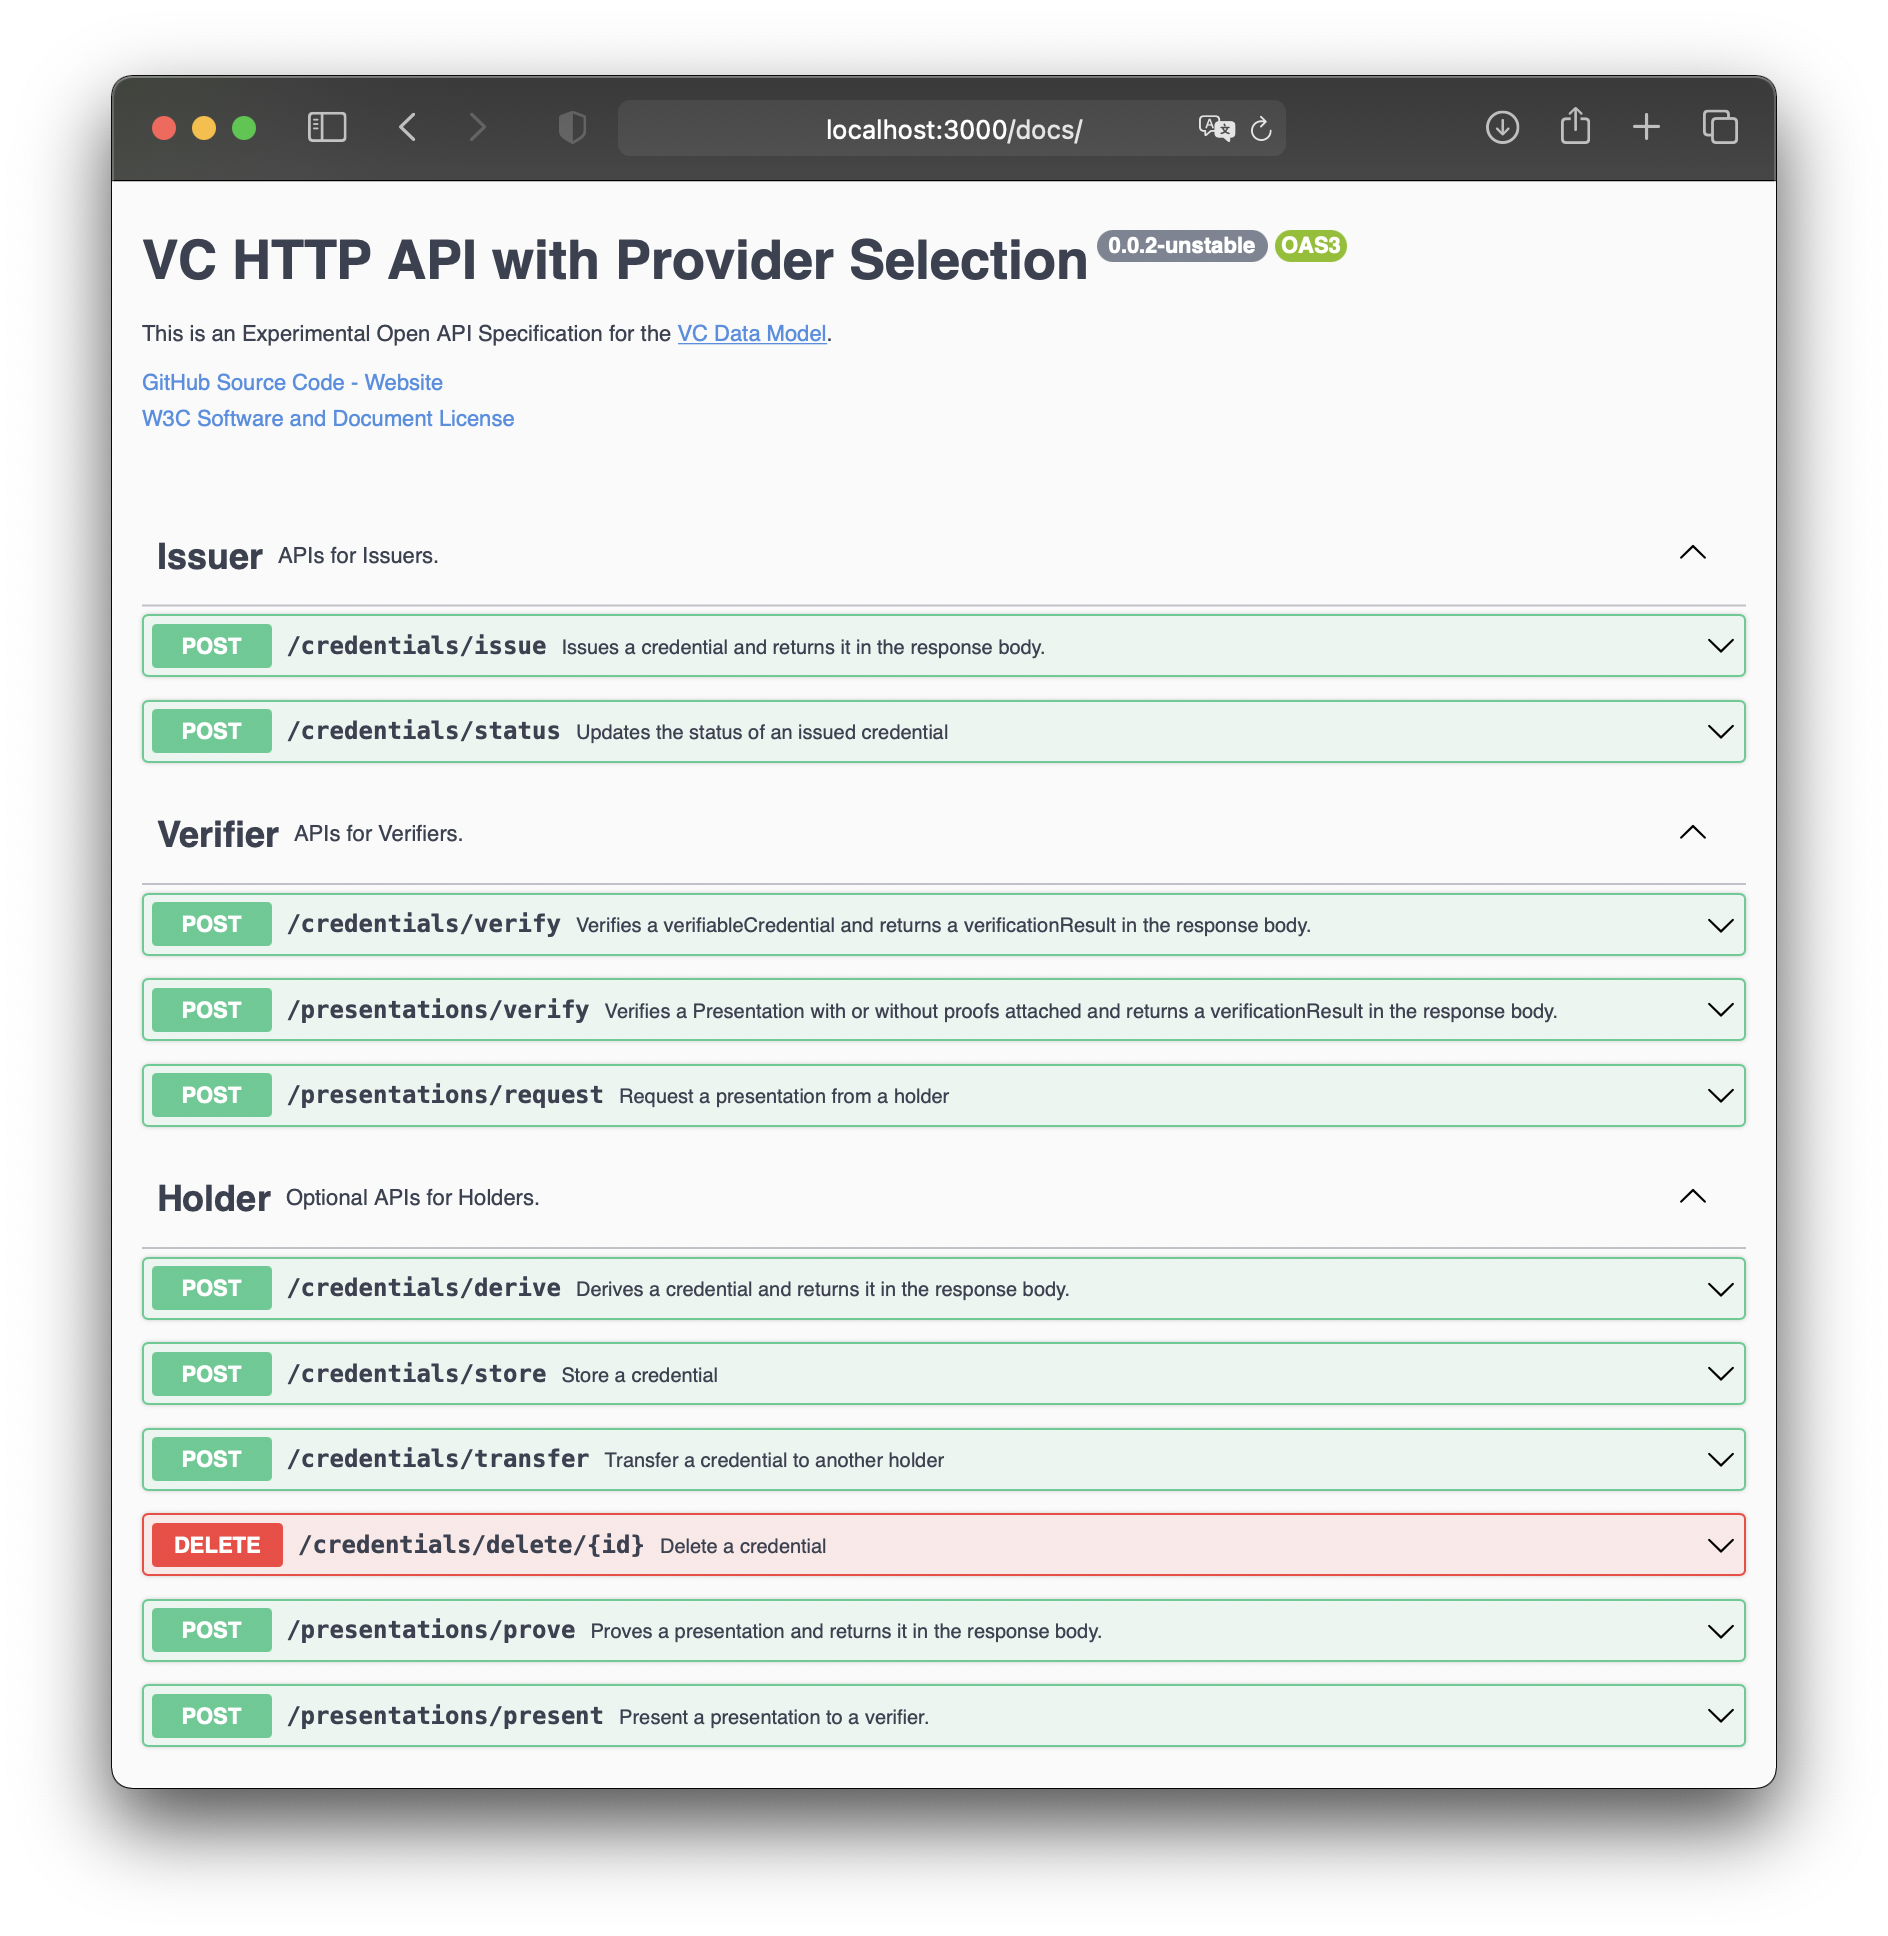
\includegraphics[width=\textwidth]{thesis/img/13_api_definition.png}}
        \caption{Modified API definition (based on \cite{world_wide_web_consortium_credentials_community_group_vc_2021})}
        \label{figure: api definition}
    \end{figure}
    
    All changes made to the original definition are summarized by the following points:
    
    % TODO: might be incomplete 
    \begin{itemize}
        \item \textit{Provider selection}: Since four providers should be addressable via the API, a query parameter was added to each route, which is based on a custom provider schema definition. Thus, it is possible to specify which provider should handle a request.
        \item \textit{Destination selection}: Another query parameter allows defining whether a request targets the local or a remote agent. This mainly includes the issuing route for a \ac{vc}, which allows a \ac{vc} to be sent directly to the subject's agent via DIDcomm or QR code. In other cases, such as transferring \acp{vc}, presenting or requesting presentations, this can be done directly via the request body. For this purpose, the schema \texttt{GenericMessage} was defined, which in its structure is very roughly based on the DIDComm data model with only the most necessary fields.
        \item \textit{Added routes}: To complete the lifecycle coverage, a route to create a presentation request has been added to the verifier, as well as routes to save, delete, transfer \acp{vc} and presenting \acp{VP} to the holder. For the request and response bodies, existing schemas were reused as much as possible.
        \item \textit{Response bodies}: Since some response bodies contained too many unnecessary attributes for the requirements of the API, the schema \texttt{GenericResult} was introduced, which only describes whether the operation was successful and whether there were errors. This schema is used for verifying, storing, deleting, and transferring \acp{vc} and verifying, as well as requesting/ presenting \acp{VP}.
    \end{itemize}
    
    The goal of the customizations was to ensure that the original API definition did not constrain the implementation, while retaining fundamental parts of the community work. Figure \ref{figure: api definition} shows on the one hand all defined routes, but also that they have been divided into the different roles. This concept was also reused for the implementation by dividing the routes into \texttt{HolderRoutes.ts}, \texttt{VerifierRoutes.ts}, and \texttt{IssuerRoutes.ts}. These implement the code for the routes they contain by accessing the provider classes generated by the factory. Further descriptions of the design patterns built on top of these are discussed in more detail in the next section. 

    % VC lifecycle -> vc-http-api -> Anpassungen -> Routen -> Aufbau/ Files
        
    \section{Factory}
    
    As already mentioned in section \ref{section: core principles}, the factory method and singleton design patterns were chosen for the software architecture. Factory method belongs to the creational patterns and thus influences how the instantiation process is carried out. A developer can thereby decide independently of the system how objects are created, which enables a high degree of flexibility. It defines an interface or an abstract class for the creation of objects, whereby the instantiation of objects is done by subclasses instead of a class. This is useful, for example, if a class does not yet know which objects it needs to create at runtime. \cite[pp. 81, 85, 107-108]{gamma_design_1995} 
    
    This pattern is appropriate because a request determines which solution and thus which objects have to be created. In addition, it allows the complexities of the individual solutions to be abstracted away, so that when defining the individual routes, only the concrete factory class must be called, which returns the correct object of the requested solution. This way, the routes only need to be programmed once and additional solutions can be added afterwards without having to change the code of the routes. Figure \ref{figure: factory method} shows a UML diagram that represents the concrete factory method pattern in the reference implementation. The interface \texttt{Factory} defines a method \texttt{createProvider()}, which is implemented by the class \texttt{ServiceProviderFactory}. This is the class which is instantiated, for example, in the routes and which is used to retrieve the object of a provider. A provider is the class of one of the four solutions that implements basic methods like the \ac{vc} issuance defined by the \texttt{ServiceProvider} interface.
    
    \begin{figure}[ht]
	    \centering    	    \makebox[\textwidth]{\includesvg[inkscapelatex=false, width=0.8\textwidth]{img/14_uml_ref.svg}}
        \caption{Factory method pattern in reference implementation (extracted and edited from \cite[p. 107]{gamma_design_1995})}
        \label{figure: factory method}
    \end{figure}
    
    As opposed to this, the singleton pattern is used in the individual concrete provider classes and allows that only one globally callable instance of a provider class can be created \cite[p. 127]{gamma_design_1995}. The rationale for this is that no more than one object is needed, caching is simplified, and multiple provider objects could lead to unforeseen complications, especially in messaging flows. 
    
    How these design patterns were implemented in the reference implementation can be seen as an example in the following listings. The starting point for the example is a route for verifying a \ac{vc} in the \texttt{VerifierRoutes.ts}, seen in listing \ref{listing: verifier routes}.
    \newline

    \begin{lstlisting}[style=ES6, caption=Extract of verifier routes, label={listing: verifier routes}]
const router = express.Router();
const factory = new ServiceProviderFactory();
router
  .post("/credentials/verify", providerCheck, async(req, res) => {
    const query = req.query.provider.toUpperCase();
    const body = req.body.verifiableCredential;
    const provider = factory.createProvider(ServiceType[query]);
    const result: GenericResult =
      await provider.verifyVerifiableCredential(body);
      
    if (result instanceof Error) {
      res.status(500).send(<GenericResult>{ 
        success: false, 
        error: result.message 
      });
    } else {
      res.status(200).send(result);
    }
  })
  ...
export = router;
\end{lstlisting}

    Here, the POST method for verifying a \ac{vc} is attached to the \texttt{router} (line 4). A \texttt{providerCheck} is appended as middleware, which checks whether the provider specified in the query is indeed valid. Within the route body, the provider object is created via the \texttt{ServiceProviderFactory}, which should handle the request (line 7). This object is then used in lines 9 to verify the \ac{vc} in the request body, the result of which is then sent as a response to the requester. By exporting the router object (line 21), all injected routes can be imported into \texttt{index.ts} and made available. This example shows that no provider-specific code is present in the route code due to the factory method pattern. To demonstrate how the \texttt{ServiceProviderFactory} works, its code can be seen in listing \ref{listing: factory}.
    \newline
    
    \begin{lstlisting}[style=ES6, caption=Extract of service provider factory, label={listing: factory}]
export class ServiceProviderFactory implements Factory {
  createProvider(type: ServiceType): ServiceProvider {
    switch (type) {
      case ServiceType.VERAMO:
        return VeramoProvider.getInstance();
      case ServiceType.Mattr:
        return MattrProvider.getInstance();
      case ServiceType.TRINSIC:
        return TrinsicProvider.getInstance();
      case ServiceType.AZURE:
        return AzureProvider.getInstance();
      default:
        return null;
    }
  }
}
\end{lstlisting}

    The class \texttt{ServiceProviderFactory} implements the \texttt{createProvider} method according to the \texttt{Factory} interface. If this method is called with the desired provider (ServiceType), as e.g. in listing \ref{listing: verifier routes} line 7, the singleton object corresponding to the provider is returned via a switch statement. According to the factory method pattern, all provider classes implement the \texttt{ServiceProvider} interface and its signatures as concrete methods. This can be seen exemplarily in listing \ref{listing: provider}.
    \newline

\begin{lstlisting}[style=ES6, caption=Example of provider implementation, label={listing: provider}]
export interface ServiceProvider {
  deleteVerifiableCredential(identifier: string): 
   Promise<CredentialDeleteResult>;
  ...
}

export class VeramoProvider implements ServiceProvider {
  async deleteVerifiableCredential(identifier: string): 
   Promise<CredentialDeleteResult> {
    const db = new VeramoDatabase();
    const result: CredentialDeleteResult = { isDeleted: false };
    try {
      const isDeleted = await db.deleteCredential(identifier);
      result.isDeleted = isDeleted[0];
      result.message = isDeleted[1];
      return result;
    } catch (error) {
      return error;
    }
  }
  ...
}\end{lstlisting}

    In this case, the class \texttt{VeramoProvider} implements the interface \texttt{ServiceProvider} with its signatures like \texttt{deleteVerifiableCredential()} concretely, to delete a \ac{vc} from the Veramo agent database.
    
    Now that the factory layer itself and how it acts as a mediator between the other layers has been described, the next section will focus on the concrete integration of the selected providers and its resulting architecture.
    
    % Designmuster weiter erklären + Vorteile -> Implementierung im Projekt
        
    \section{Provider Integration}
    
    Having looked at the general architecture and its concrete implementations concerning routes and abstractions, this section focuses on the integration of the individual providers. For this purpose, figure \ref{figure: sys architecture} shows the concrete architecture of the reference implementation, which is based on the previously defined reference architecture. 
    
    \begin{figure}[ht]
        \centering
        \makebox[\textwidth]{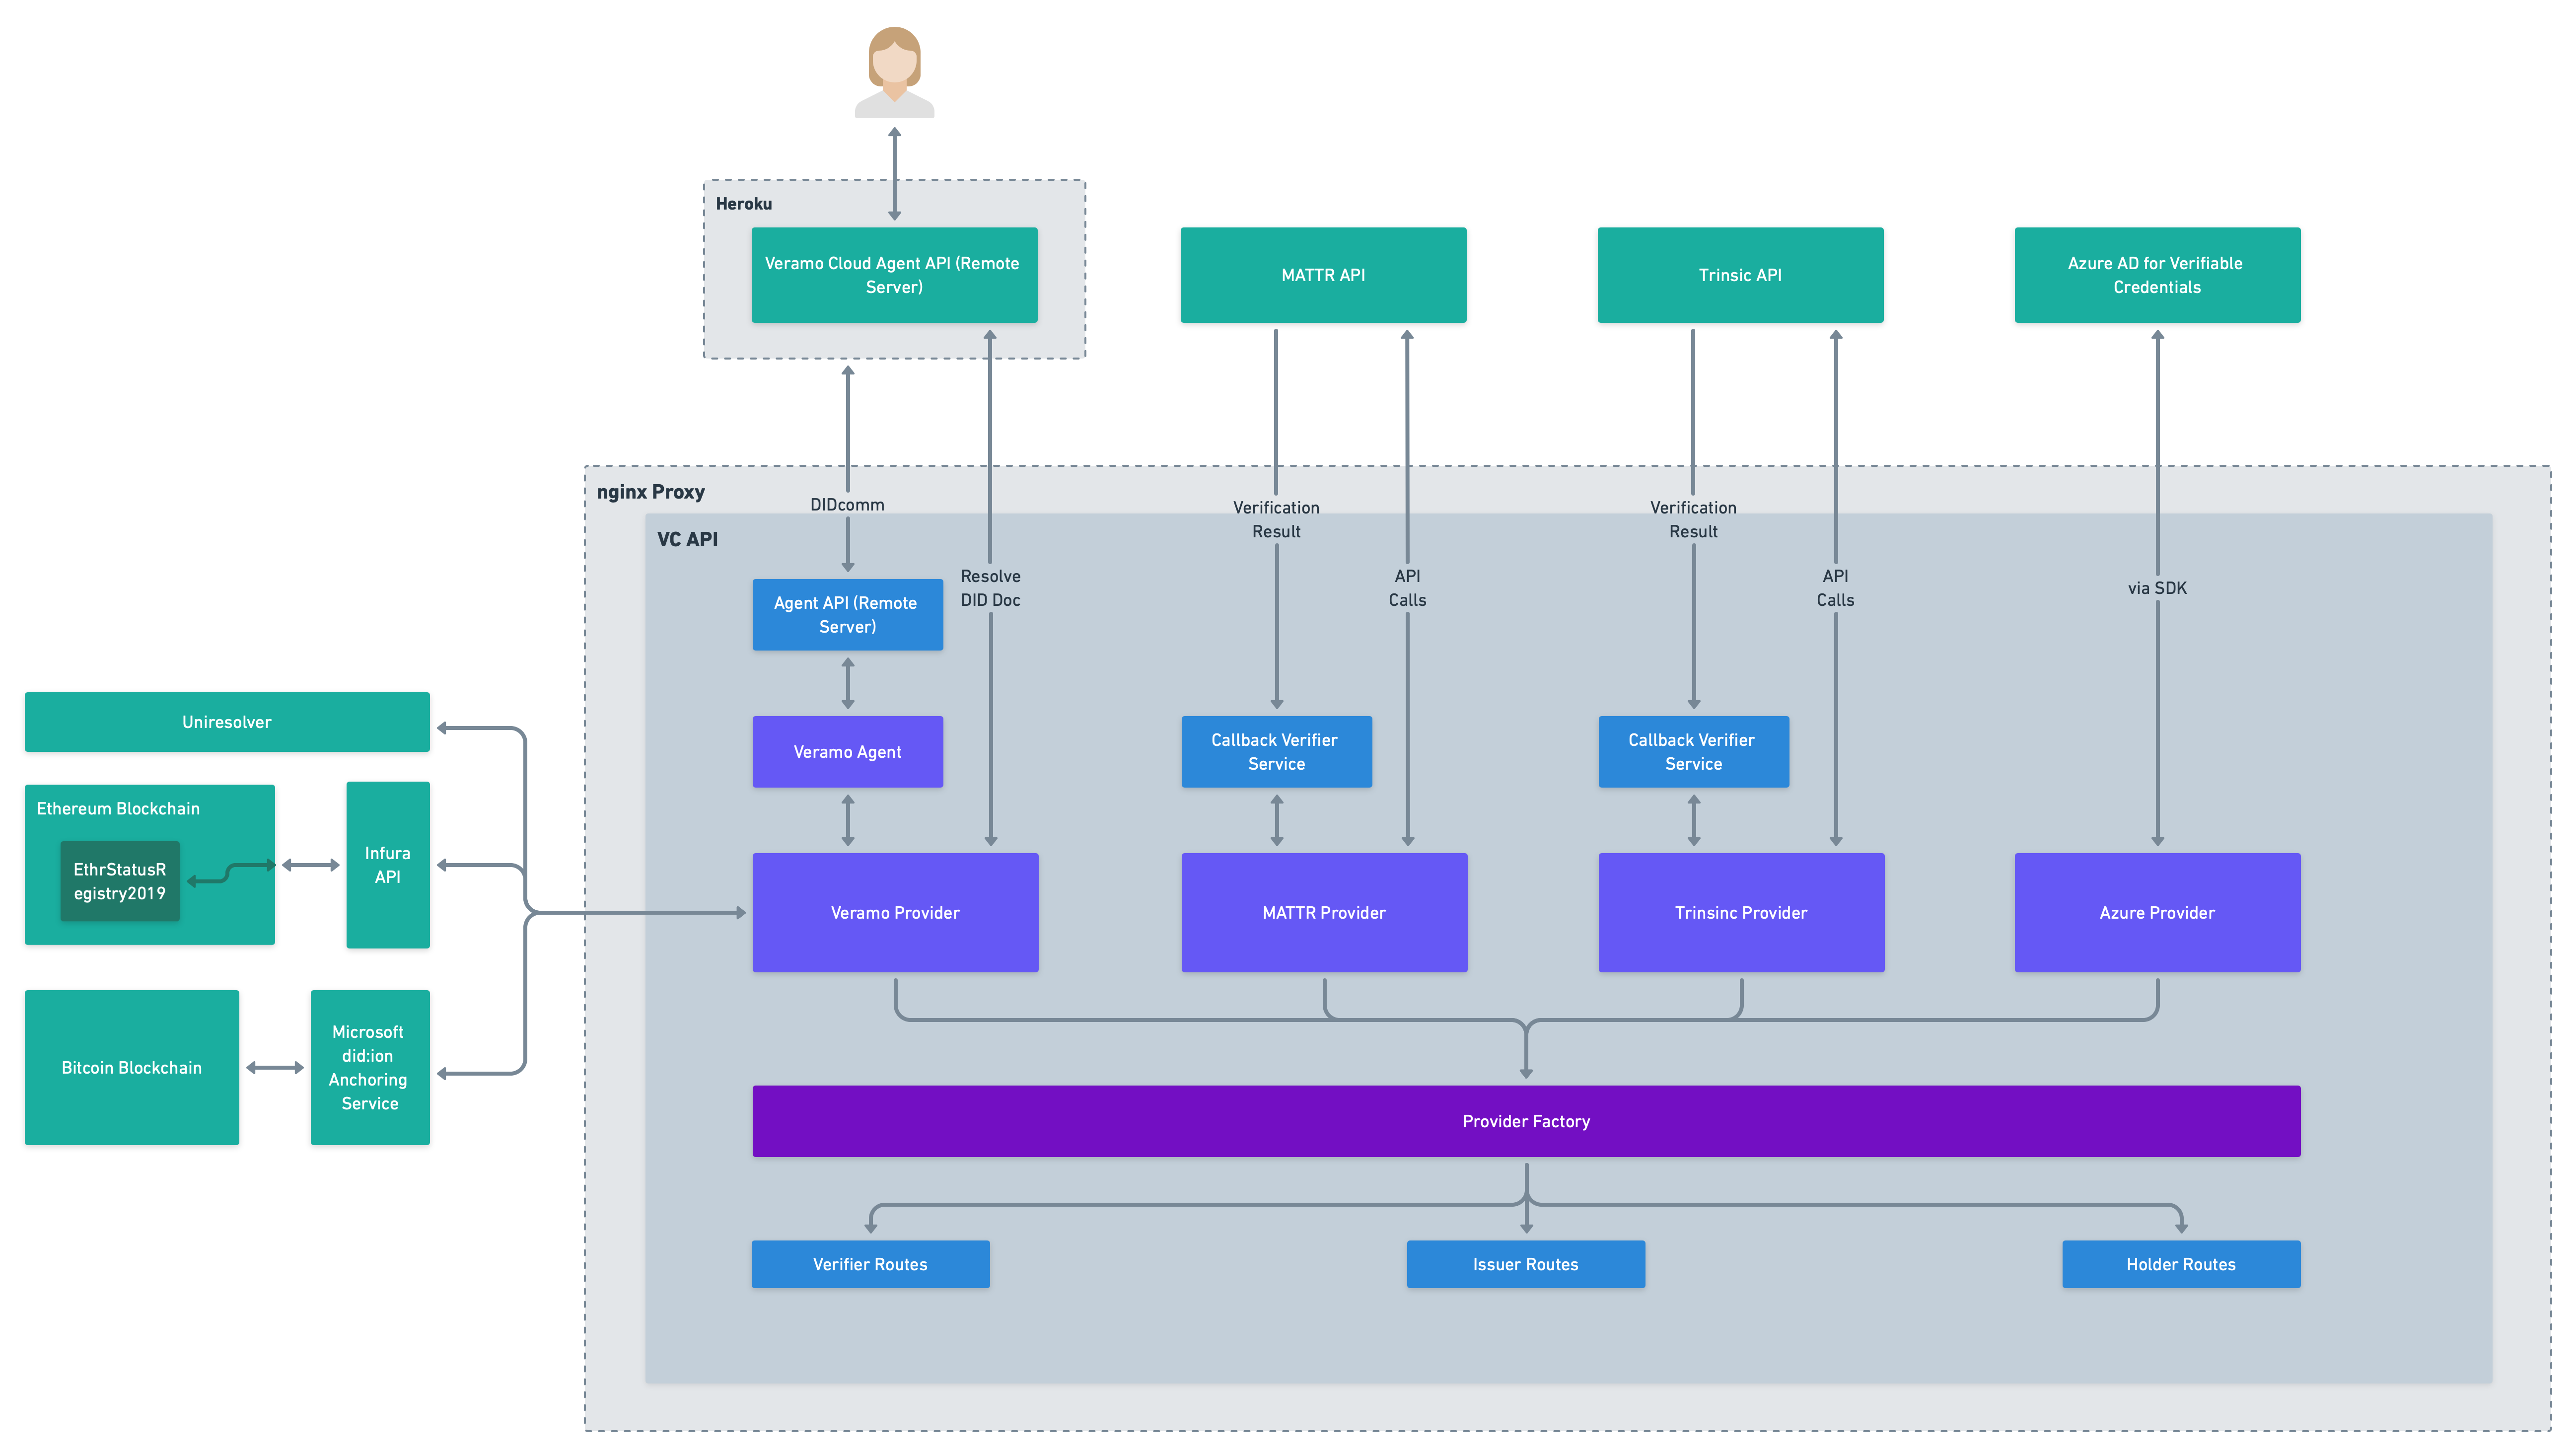
\includegraphics[width=\textwidth]{thesis/img/15_architecture.png}}
        \caption{System architecture (TODO: Vector redo)}
        \label{figure: sys architecture}
    \end{figure}
    
    This contains the previously defined types of routes at the bottom, but also the provider factory and the four providers above it. Added at this point are mainly provider-specific elements like callback services, but also an nginx proxy that surrounds the reference implementation. This proxy is assigned a domain so that external components can correctly address internal components such as callback or messaging services. The specific provider implementations, its peculiarities and gained experiences will be discussed in more detail in the next subsections for each provider.
    
        % fka Solution Integration
        \subsection{Mattr}
        
        With regard to the integration of the Mattr provider into the reference implementation, the generous free tier and the well-structured documentation proved to be helpful. Thus, a large part of the \ac{vc} lifecycle could be integrated relatively unproblematically by simply addressing the corresponding endpoints of the Mattr REST API. These take care of any logic and can be used to manage \acp{DID}, their keys, \acp{vc}, \acp{VP}, revocation lists, as well as presentation templates. The support of BBS+ for \ac{ZKP} credentials, revocable credentials (RevocationList2020) and LD proofs is directly integrated into the platform as well. For mobile wallet interactions concerning \ac{vc} issuance, an \ac{OIDC} provider (see subsection \ref{subsection: user centric}) like Auth0 was necessary at the time of implementation. Its initial setup took some time, but was feasible due to the good documentation. By now, \acp{vc} can also be issued directly using Mattr's \ac{JWM} module, QR codes, or deep links to the Mattr mobile wallet without an \ac{OIDC} provider. With regard to presentation requests and its verification results, the sample apps were used to integrate a callback service into the reference implementation, although this flow can also be implemented via \ac{OIDC} with greater effort. The Mattr team also seems to actively maintain their external Slack channel, as they are relatively quick to respond to questions and issues from platform users there, and even offer private calls in some cases. In summary, the broad coverage of the \ac{vc} lifecycle, the large number of features, and the developer-friendly documentation with tutorials stood out positively. Mattr therefore offers developers deep but simple and well-documented access to various current technologies and facets of \ac{SSI}.
    
        Nevertheless, some things were noticed that could be problematic and restrictive under certain circumstances. For example, on-boarding to the platform has been relatively cumbersome in April 2021, as it was necessary to join the official Slack channel after successful registration, where support then triggers the rest of the process manually. After the cloud agent had been created, the password was communicated by the support via Keybase. An automated process without the need for Slack and Keybase would certainly have been much more pleasant, whereas this seemed to be only an interim solution. Additionally, some features are not or only partially usable in combination, such as the support of BBS+ only for credentials based on did:key or did:ion. Finally, it should be noted that the private keys for all \acp{DID} are managed by Mattr and cannot be exported by users. This reflects the platform nature of Mattr, which does not allow developers to extend basic functionality. If the existing features are sufficient, this is certainly not a problem, but the resulting inflexibility can be restrictive and make custom flows impossible. So potential developers will need to look closely at whether Mattr's approach aligns with their goals and product strategy.
    
        The majority of the integration took place in \texttt{MattrProvider.ts}, which implements the \texttt{ServiceProvider} interface. Since this class implements any functionality via HTTP requests, listing \ref{listing: Mattr verification} shows how this is done in the context of directly verifying a \ac{vc} object. However, it should be noted that methods such as \texttt{issueVerifiableCredential()} are significantly more complex, as specific logic such as the distinction in issuance to a wallet or not must be considered accordingly.
        \newline

\begin{lstlisting}[style=ES6, caption=Example of Mattr verification implementation, label={listing: Mattr verification}]
async verifyVerifiablePresentation(body: VerifiablePresentation): 
 Promise<GenericResult> {
  const request = { presentation: body };
  const authToken: string = await this.getBearerToken();
  const result: GenericResult = {
   success: null,
  };

  try {
    const response = await fetch(`.../presentations/verify`, {
      method: "POST",
      body: JSON.stringify(request),
      headers: { 
        "Content-Type": "application/json", 
        Authorization: `Bearer ${authToken}` 
      },
    });
    const verificationResult = await response.json();
    result.success = verificationResult.verified;
    result.error = verificationResult.reason;
    return result;
  } catch (error) {
    return error;
  }
}\end{lstlisting}
    
    Additionally, helper methods were implemented to generate authentication tokens for communcating with Mattr's API, or to cache QR codes containg \ac{vc} issuance requests. Especially interactions with the latter required several extra implementations that enable the generation of issuance and presentation requests in the form of QR codes via an OIDC provider to Mattr. Starting with the issuance of a \ac{vc} to such a wallet, the type, and attributes of the \ac{vc} must be prepared at the OIDC provider and Mattr. The resulting provider ID can then simply be referenced in an issuance URL and, if desired, encoded in a QR code. By scanning this, the associated VC can be obtained directly in the Mattr wallet app. This logic is part of the \texttt{MattrVerifierService.ts} and can be seen in listing \ref{listing: Mattr oidc issuance}.
    \newline
    
\begin{lstlisting}[style=ES6, caption=\ac{OIDC} issuance QR code generation, label={listing: Mattr oidc issuance}]
private getOIDCIssuerQRCode(oidcIssuer: string): Buffer {
  if (this.issuerQrCache.has(oidcIssuer)) 
    return this.issuerQrCache.get(oidcIssuer).image;

  const qrcode: Buffer = qr.imageSync(
    `openid://discovery?issuer=${process.env.Mattr_URL}
    /ext/oidc/v1/issuers/${oidcIssuer}`,
    { type: "png" }
    );
  this.issuerQrCache.set(oidcIssuer, qrcode);
  return qrcode;
  }
}\end{lstlisting}

    To verify a \ac{vc} from the Mattr wallet app, a presentation request must be prepared. For this purpose, a presentation template is first defined on the Mattr platform, which contains, for example, the allowed issuers and the requested attributes of a requested \ac{vc}. Mattr assigns a unique ID to this template. This ID can then be used in the first step of provisioning in the reference implementation. Here the actual presentation request is prepared with the verifier \ac{DID}, the template ID, an expiration date and a callback URL via the Mattr API. In the next step, authentication keys are retrieved as a \ac{DID} URL from the verifier \ac{DID} document via the Mattr platform to sign the presentation request via the same platform in the next step. The resulting JWS payload is cached and a QR code is generated with a public URL of the reference implementation. This process can be seen in listing \ref{listing: Mattr oidc presentation}.
    \newline
\begin{lstlisting}[style=ES6, caption=Generate QR code for OIDC presentation reqest, label={listing: Mattr oidc presentation}]
public async generateQRCode(request: GenericMessage): Promise<Buffer> {
  const templateId: string = request.body.request.credentialType;
  
  // Check cache
  if (this.qrCache.has(templateId)) 
    return this.qrCache.get(templateId).image;

  // Prepare QR code and JWS payload URL
  const publicUrl = this.publicUrl;
  const provisionRequest = 
    await this.provisionPresentationRequest(publicUrl, request);
  const didUrl = await this.getVerifierDIDUrl(request.from)
  const didcommUrl = 
    await this.signPayload(publicUrl, didUrl, provisionRequest); 
  const qrcode = qr.imageSync(didcommUrl, { type: "png" });
    
  // Cache and return it
  this.qrCache.set(templateId, qrcode, request.expiresTime);
  return qrcode;
}\end{lstlisting}
    
        When the QR code is scanned with the Mattr wallet app, the QR route of the \texttt{MattrVerifierRoutes.ts} is called, which returns the cached JWS payload url. This is the starting point for all further interactions between the wallet app and the Mattr platform. The callback route (callback verifier service in figure \ref{figure: sys architecture}) in the reference implementation allows Mattr to report whether the presentation was successful and the \ac{vc} could be verified. Both routes were defined via the express router.
        
        Finally, six out of ten method signatures of the \texttt{ServiceProvider} interface could be implemented directly, whereas all functionalities except the transfer of \acp{vc} are at least indirectly part of the platform. In the next subsection, Trinsic will be discussed in the same context.
    
        \subsection{Trinsic}\label{subsection: trinsic}
        
            The integration of Trinsic into the reference implementation proved to be pleasant. This was mainly due to the documentation but also due to their Trinsic Studio. With the latter, an organization, associated credentials, and verification templates could be created within a few minutes using a simple dashboard. This is however also possible programmatically via their API, which leaves room for automation. The resulting IDs could later be used to trigger the issuance and presentation flows using Trinsic's JavaScript SDK, which also includes type definitions for TypeScript. No other solution made the implementation process so quick and easy.
    
            The Hyperledger focus is, however, noticeable from a technological point of view. Only JSON credentials and CL signatures for revocation, DIDComm v1, Aries exchange protocols and Hyperledger-specific \ac{DID} methods like did:sov are supported. Newer technologies as well as \ac{DID} methods based on public permissionless blockchains are not supported. In addition, functionality is abstracted away even further in contrast to Mattr, which increases user-friendliness but hardly allows any flexibility. Thus, no custom \acp{DID} can be generated, and no \acp{vc} in can be directly issued or verified without first generating a template. Direct access for generating \acp{VP} on the cloud agent or the \ac{ZKP} function is also not available. All these things are managed in the background and abstracted away by Trinsic and the mobile wallet. This can certainly be sufficient for certain use cases, but maybe too inflexible for others. Just like Mattr, developers are completely dependent on Trinsic in terms of the tech stack and private key management. The company is trying to address many of the points mentioned above with the Core v2 platform, which is currently in closed beta. Latest technologies such as JSON-LD credentials, LD proofs, BBS+, presentation exchange, DIDComm v2 and new \ac{DID} methods such as did:key or did:web are supported here. Trinsic could thus catch up with Mattr in terms of supported technologies. Table \ref{tab: trinsic roadmap} shows the current roadmap of the Trinsic platform.
            \newline
    
        	\begin{center}
            \captionof{table}{Trinsic Roadmap (based on \cite{riley_hughes_announcing_2021})}
        		\begin{threeparttable}
            		  \begin{tabular*}{\textwidth}{l @{\extracolsep{\fill}} llll}
            			\toprule 
            			Type & Current & Beta & Future\tabularnewline
            			\midrule
            			\textbf{Data Exchange} & JSON & JSON-LD   & JWT \tabularnewline
            			\textbf{}              & CL signatures    & BBS+ signatures       & OIDC SIOP\tabularnewline
            			\textbf{}              & Aries exchange   & Presentation exchange & \tabularnewline
            			\textbf{Communication} & did:peer         & did:key               & WACI\tabularnewline
            			\textbf{}              & DIDComm v1       & DIDComm v2            & BLE, NFC\tabularnewline
            			\textbf{}              & HTTP transport   & gRPC transport        & \tabularnewline
            			\textbf{Public Trust}  & did:sov          & did:key, did:web      & did:un, did:ion\tabularnewline
            			\textbf{}              & Hyperledger Indy & did:indy              & \tabularnewline
            			\bottomrule 
            		\end{tabular*}
        	\end{threeparttable}
        	\label{tab: trinsic roadmap}
    	\end{center}
    	
        The main part of the implementation takes place in the \texttt{TrinsicProvider.ts}, which implements the \texttt{ServiceProvider} interface. To communicate with the Trinsic API, the JavaScript SDK was used to create an object of the \texttt{CredentialsServiceClient} class. This is done in the constructor so that the object is available immediately after initialization. This can be seen in listing \ref{listing: trinsic service client}.
    \newpage
    \begin{lstlisting}[style=ES6, caption=Connecting to Trinsic API via SDK, label={listing: trinsic service client}]
export class TrinsicProvider implements ServiceProvider {
  client: CredentialsServiceClient;

  private constructor() {
    this.client = new CredentialsServiceClient(
      new Credentials(process.env.TRINSIC_KEY), 
      { noRetryPolicy: true }
    );
  }
  ...
}\end{lstlisting}
    
    How to programmatically issue a \ac{vc} to the mobile wallet via Trinsic, for example, can be seen in listing \ref{listing: trinsic issuance}. As required by the \texttt{ServiceProvider} interface, this is done by implementing the \texttt{issueVerifiableCredential()} method that first checks whether the requester actually wants to issue a pre-defined credential to the wallet. If this is not the case, it is informed that only predefined credentials can be issued to a wallet. If everything is correctly defined, the ID of the credential template as well as the values for the attributes of the credential are obtained from the request body. The \texttt{GenericMessage} schema in the request body is used for this. An object is formed from these values, which is submitted to the API via the Trinsic SDK and results in a \texttt{CreateCredentialResponse} object. The \texttt{offerUrl} contained therein is then encoded in a QR code, which can then be scanned via the Trinsic wallet to retrieve the \ac{vc}. 
    \newline
    
    \begin{lstlisting}[style=ES6, caption=\ac{vc} issuance with Trinsic, label={listing: trinsic issuance}]
async issueVerifiableCredential(
  body: IssueCredentialRequest | GenericMessage,
  toWallet: boolean
): Promise<IssueCredentialResponse | Buffer> {
  try {
    if (!toWallet) throw Error("Only issuance to Trinsic wallet...");
    if (isGenericMessage(body)) {
    
      // Prepare request body for Trinsic
      const message: GenericMessage = body;
      const request = {
        definitionId: message.body.credentialType,
          connectionId: null,
          automaticIssuance: false,
          credentialValues: message.body.claimValues,
      };
      
      // Generate QR code with offer URL
      const vcOffer: CreateCredentialResponse = 
        await this.client.createCredential(request);
      const qrcode: Buffer = 
        qr.imageSync(vcOffer.offerUrl, { type: "png" });
        
      return qrcode;
    } else {
      throw Error("Issuing manual VCs is not supported...");
    }
  } catch (error) {
    return error;
  }
}\end{lstlisting}

    In the case of Trinsic, three of ten signatures of the \texttt{ServiceProvider} interface could be implemented directly, while all parts except for the transfer of \acp{vc} are at least indirectly part of Trinsic. Among them are the methods for issuing, deleting and creating presentation requests. The method for revoking credentials could have been implemented theoretically, but was not part of the free tier. After a presentation request has been successfully performed by the user, the result of the verification can be received via a webhook in the reference implementation. Similar to Mattr, a route was created via Express, to which the Trinsic platform can send the result. This webhook URL also had to be added via the Trinsic Studio beforehand, since the URL is not part of the presentation request body, as opposed to Mattr. Listing \ref{listing: trinsic webhook} shows how the webhook route is implemented. This forms, together with the verification method, the callback verifier service as shown in the system architecture in figure \ref{listing: trinsic webhook}.
    \newline
    
    \begin{lstlisting}[style=ES6, caption=Trinsic webhook for verification result, label={listing: trinsic webhook}]
const router = express.Router();
const trinsic = TrinsicProvider.getInstance();

router.post("/webhook", async (req, res) => {
  try {
    if (req.body.message_type === "verification") {
      const verification = 
        await trinsic.client.getVerification(req.body.object_id);
      console.log(verification);
    }
  } catch (error) {
    console.log(error.message || error.toString());
  }
  res.status(200).end();
});

export = router;
\end{lstlisting}

        At this point, all the specifics of the Trinsic platform and its integration into the reference implementation have been addressed. In the next subsection, Veramo's implementation will be presented.
    
        \subsection{Veramo}
        
        The integration process of Veramo into the reference implementation proved to be a mixed experience. Especially the \ac{CLI} offered a good first start to try out Veramo. Thus, all features like creating \acp{DID}, issuing, verifying, and requesting \acp{vc} could be tested in advance without any implementation process. Within the implementation, the very high degree of flexibility was especially noticeable. None of the previous solutions supports this amount of \ac{DID} methods (did:key, did:web, did:ethr, did:ion), whereas the connection to the Uniresolver allows resolving almost any \ac{DID}. In terms of deployment options, the Veramo agent can be used in web frontends, smartphone apps, and backend systems through the TypeScript backend, while the agent's modularity also allows tasks to be distributed among different agents. This allows for different architectures where, for example, one Veramo cloud agent implements only key management, another implements the issuing of \acp{vc}, and the agent in the mobile wallet implements only messaging and credentials storage. Since the Veramo agent also exposes all of its functionalities via a REST API with OpenAPI documentation, similar to Mattr and Trinsic, all functions can also be used on non-supported platforms via HTTP requests. This is not possible with any of the other solutions. In addition, with the DIDComm v1 implementation, complex communications between Veramo agents could also be implemented, such as the transfer of credentials between holders. Because of the open access to these modules, pretty much any use case can be realized, which is not possible due to limitations in the other solutions. Since the integration, Veramo released a DIDComm v2 module which replaces the old alpha version of DIDComm v1 \cite{veramo_blog_2021}.
        Especially for messaging cases, it was very helpful that a Veramo agent could be created on Heroku with a one-click button, making such multi-agent flows testable without many preparations. In addition, the React Native integration was tested, with which a demo mobile wallet was created in a short time to test the management of \acp{vc} and messages. 
        In contrast to the platform solutions, the flexibility but also the complete control over architecture, flows, code, and data such as the \acp{vc} and the private keys of \acp{DID} stand out. 
    
        Nevertheless, there were a few things that complicated the implementation process. The now updated documentation was either outdated or not available at all in April 2021. Only the code of the \ac{CLI} implementation could be used as a guide, which in combination with some guesswork and trial and error led to the desired goal. Even today, not all areas and features are covered so far, such as code and explanations for the messaging system, how to issue and verify credentials, how to resolve \acp{DID}, that there is a did:ion plugin, types of events in the event system and much more. The documentation really only covers the most necessary areas to get started, which may discourage some developers. Furthermore, there are some technological limitations, which are briefly listed below:
    
\begin{itemize}
    \item \textit{Credential type}: Currently only JWT credentials are supported. Support for JSON-LD signatures is currently being worked on \cite{terbu_tracking_2021}.
    \item \textit{Revocation}: There are no official, up-to-date plugins for revocation. There is only a library from two years ago that can be used with manual effort in Veramo to create revocable credentials with did:ethr and later revoke them as well. Support for RevocationList2020 does not exist, but can be retrofitted with open libraries from Digital Bazaar due to Veramo's open architecture.
    \item \textit{Selective Disclosures \& \ac{ZKP}}: Due to the nature of JWT credentials, this is not currently possible. Veramo recommends keeping credentials as atomic as possible so that the user can present individual credentials with only a few attributes. Additionally, Veramo currently uses a proprietary exchange data format instead of the DIF Presentation Exchange format. However, support for BBS+ in combination with LD proofs and Presentation Exchange is planned \cite{terbu_tracking_2021}.
    \item \textit{Verification}: There is no proper API for verifying \acp{vc} and \acp{VP}. Meanwhile, only the validity of the JWT can be checked, but this does not retrieve the \ac{DID} document for the issuer's public key, does not check for revocation, integrity, or other important parameters. The developer currently has to check all of these by itself. However, this is also being looked at by the development team, which is working on a comprehensive verification API \cite{riedel_generalized_2021}.
\end{itemize}

    This makes it clear that Veramo really is a beta and that various areas are not yet ready. Nevertheless, it should be noted that, in contrast to the other solutions, the open architecture means that missing functions can be retrofitted at any time. This behaviour is also supported by the Veramo developers, as they want an ecosystem of community plugins.
    
    Looking at the reference implementation, there is more effort here compared to the platform solutions, as now any logic has to be implemented via the Veramo API itself. In the middle of this is the \texttt{VeramoProvider.ts}, which implements the \texttt{ServiceProvider} interface and thus all lifecycle-specific methods. In order to access the methods of the Veramo API and its included plugins, an object of the Veramo agent is created and exported in the \texttt{VeramoSetup.ts} so that it can be directly imported and used in various places. To create the agent, all necessary plugins must be imported in the form of libraries and taken into account when initializing the object. This can be seen exemplary in listing \ref{listing: veramo agent}. 
    \newline
    \begin{lstlisting}[style=ES6, caption=Veramo agent creation, label={listing: veramo agent}]
// Core interfaces
import { createAgent, IDIDManager, ... } from "@veramo/core";

// Core identity manager plugin
import { DIDManager } from "@veramo/did-manager";

// Credential Issuer
import { CredentialIssuer, ICredentialIssuer } from "@veramo/credential-w3c";

...

export const veramoAgent = createAgent<
  IDIDManager & IKeyManager & IDataStore & IResolver & ... >({
  plugins: [
    ...
    new KeyManager({
      store: new KeyStore(dbConnection, new SecretBox(secretKey)),
      kms: {
        local: new KeyManagementSystem(),
      },
    }),
    new DIDManager({
      store: new DIDStore(dbConnection),
      defaultProvider: "did:key",
      providers: {
        "did:key": new KeyDIDProvider({
          defaultKms: "local",
        }),
        ...
      },
    }),
    new DIDResolverPlugin({
      resolver: new Resolver({
        ...
        key: getDidKeyResolver().key,
        ...getUniversalResolverFor(["io", "elem", "sov"]),
      }),
    }),
    new CredentialIssuer(),
    new MessageHandler({ ... }),
    ...
  ],
});\end{lstlisting}
    
    This is only a small excerpt, but it demonstrates the rough concept and functionality. For the reference implementation, various plugins were implemented for storing and managing keys, \acp{DID}, \acp{vc}, \acp{VP} as well as messages, message handlers (DIDComm, JWT, ...), \ac{DID} providers, \ac{DID} resolvers and credential issuance. In addition, event listeners were utilized to document verification results and submitted presentation requests. Especially the latter was helpful in testing the multi-agent messaging flows to let a cloud agent automatically respond to submitted presentation requests via its API. This part is relatively well documented, but there were problems implementing the message handlers correctly, which resulted in errors with the validation of messages like JWT credentials or DIDComm messages. The author's issue report on GitHub was answered by the Veramo developers on the same day. It was described that the order in which the different message handlers are integrated in the setup is significant and was incorrect in the reference implementation. Such small details are unfortunately not documented and cost considerable time to debug. That being said, the author was able to identify an actual bug during implementation where mismatches of signatures between a \ac{vc} and its \ac{VP} occur under certain circumstances. This report was also being responded to on the same day and a fix was rolled out in under two weeks. The developers appear to respond quickly and helpfully in general on GitHub.
    
    With regard to the actual implementation of the lifecycle in the \texttt{VeramoProvider} class, the methods of the Veramo agent proved to be well usable. Basic methods for creating \acp{vc}, \acp{VP}, verifying messages like JWT credentials and sending presentation requests are provided, the latter being called Selective Disclosure Requests by Veramo. Looking at the descriptions of this topic in subsection \ref{subsection: bbs} and the nature of JWT credentials, the term selective disclosure is not well-chosen, since only a set of credentials and not a set of attributes of one credential are disclosed here. In listing \ref{listing: veramo issuance} is a code snippet for creating a \ac{vc} using the Veramo agent.
    \newline
        \begin{lstlisting}[style=ES6, caption=Issue a \ac{vc} with Veramo, label={listing: veramo issuance}]
async issueVerifiableCredential(body: IssueCredentialRequest, 
 toWallet: boolean): Promise<IssueCredentialResponse> {
    try {
      body.credential.issuer = { id: body.credential.issuer.toString() };
      const save: boolean = body.options.save ? body.options.save : false;
      const credential: W3CCredential = body.credential;
      
      const verifiableCredential: W3CCredential = 
       await veramoAgent.createVerifiableCredential({
        save: false,
        credential,
        proofFormat: "jwt",
      });

      // Prepare response
      const result: IssueCredentialResponse = {
        credential: verifiableCredential,
      };

      if (toWallet) {
        try {  // Send VC to another Veramo agent
          const msg = await veramoAgent.sendMessageDIDCommAlpha1({
            save: true,
            data: {
              from: verifiableCredential.issuer.id,
              to: verifiableCredential.credentialSubject.id,
              type: "jwt",
              body: verifiableCredential.proof.jwt,
            },
          });
          result.sent = true;
          return result;
        } catch (error) {
          return error;
        }
      }
      return result;
    } catch (error) {
      return error;
    }
  };\end{lstlisting}
    
        At the beginning, the credential object is prepared, which is then converted to a \ac{vc} in lines 8 to 13 using the methods. After that, the API response is prepared with the created \ac{vc}, or if an error occurs during issuance, the error is sent directly to the requester as a response. If the request to the API defined that the \ac{vc} should be sent directly to the agent of the \ac{DID} via the messaging endpoint, lines 21 to 35 handle this using the \texttt{sendMessageDIDCommAlpha1()} method. This method has been deprecated and should be replaced by the new DIDComm v2 implementation. Considering the scope of this work, a short-term implementation of the new module has been omitted at this point. This feature is useful, for example, to send a \ac{vc} directly to the Veramo agent of a mobile wallet. Mattr and Trinsic offer similar functions as an alternative to scanning QR codes.
    
        In addition, four other files and classes were created to implement or retrofit Veramo-specific features. These are briefly described below:
    
        \begin{itemize}
            \item \textit{VeramoDatabase.ts}: At the time of development, there was no method to delete \acp{vc} from the local flatfile database. Since the database is in the sqlite format, the \texttt{sqlite3} library was used to add that functionality. Since v2.1.0 this is also a native DataStore functionality.
            \item \textit{VeramoRevoker.ts}: This class implements uPort's \texttt{ethr-status-registry} library and retrofits the functionality to revoke an \ac{vc} with a did:ethr within an on-chain smart contract on the Ethereum Blockchain. This requires a connection to an Ethereum node or a service provider such as Infura.
            \item \textit{VeramoRemoteAgent.ts}: This class can connect to another Veramo agent that one has control over. This is more of a helper class that can be used for testing purposes, for example, to force a cloud agent to automatically respond to a presentation request via its RESTful API.
            \item \textit{VeramoAgentAPI.ts}: Here, the local Veramo agent exposes its methods via a RESTful API and the associated API docs. Furthermore, a did:web is automatically set up for the external URL and the associated messaging endpoint. This is relevant for multi-agent communication flows.
        \end{itemize}
    
        Flexibility and liberty are the main advantages of Veramo, yet the beta status was noticeable during the implementation. Some central features are not or only partially available, and from the descriptions about it is clear that a lot is happening. Within a few months, some features were added that made some implementations (see VeramoDatabase.ts, DIDComm) obsolete. Thus, nine out of 10 methods could be implemented directly, although with technical limitations. In the next subsection, Azure AD for Verifiable Credentials will be discussed as the last of the four solutions. 
    
        \subsection{Azure}
        
        With regard to the implementation, in contrast to Mattr and Trinsic, the platform consisting of Active Directory and additional components still had to be prepared. Since the extension for Verifiable Credentials is still in public preview, a P2 licence is required, which is associated with higher costs. Alternatively, a developer account can be requested from Microsoft. Within the client a new resource group is created, which must contain a key vault for keys, a storage account for credential specific rules and display JSON files and various other settings. Microsoft provides detailed documentation with descriptions and illustrations for these steps, so this process was fairly straightforward. Nevertheless, this can definitely be confusing in some places for Azure beginners. In the next step, the actual Verifiable Credential can be defined in its content and representation, which is also described in the documentation. Azure automatically assigns a URL to this \ac{vc} schema, which means that it can be retrieved via an OpenID provider. There are other steps, such as creating an application in Azure so that issuance and verification can take place in the reference implementation. Positive was the good and clear documentation to prepare a client to issue and verify \acp{vc}. Furthermore, it is certainly interesting for companies that already use Microsoft products and Active Directory. The \ac{vc} solution could be integrated into existing architectures without much effort. Moreover, it is one of the few solutions that uses ION as the \ac{DID} method, relying on a public permissionless blockchain, thus actually creating independent \acp{DID} that can also embed metadata in their \ac{DID} documents. With Azure, \acp{vc} can be issued to the mobile app in JWT format and also presented from there as a \ac{VP} on the basis of a corresponding request. In addition, \acp{vc} can be revoked through the Azure portal.  
    
        Nevertheless, there are some points that make the Microsoft solution appear incomplete, and lack transparency compared to the other solutions. For example, Azure abstracts various logic and complexities similar to Trinsic, with the difference that even fewer features are available, and it is even less clear which standards are used at which point. Through debugging sessions of the author, it was possible to determine that simple JWT credentials are exchanged and propriety revoking mechanisms are used. Moreover, unlike Mattr and Veramo, \acp{vc} cannot be issued and verified directly based on a JSON-LD input either, which means that only \acp{vc} whose schema has been defined in Azure beforehand can be issued or verified. In addition, there appears to be no official API for revoking credentials yet, which is why it was not possible to implement this in the reference implementation. Furthermore, routes for storing, verifying, and presenting without request could not be implemented because no APIs are offered for this. These steps are abstracted away in other process steps, while the transfer and derivation for \acp{ZKP} of \ac{vc} is not possible at all. Due to the missing functionalities, it is impossible to implement the complete lifecycle with its individual steps. In addition, the example projects with code for issuers and verifiers are functional but not documented at all, which led to some confusion. Furthermore, basic type definitions for TypeScript seem to be flawed and even so the code seems to be questionable. There was a GitHub issue \cite{yegupov_demo_2021} about this, which the author of this work also responded to, and was eventually closed without comment by the repository owner. The original creator of the issue announced that they ultimately decided against the Azure solution. With correspondingly messy modifications, functionalities for issuance and presentation request routes could still be implemented. Additional \ac{DID} methods, revocations standards, \ac{ZKP} technologies such as BBS+ and associated LD proofs have not been announced. In terms of the basic approach, Microsoft's solution is most similar to Trinsic, but is not on a par in terms of functionality, documentation, SDKs and associated examples.

        The main part of the implementation takes place in \texttt{AzureProvider.ts}, which implements the \texttt{ServiceProvider} interface. Unique aspects are that at the beginning of the class, an object of the \texttt{CryptoBuilder} class of the verifiablecredentials-verification-sdk-typescript library and a request cache are created as \texttt{Map<string, any>}. The former can be used to create the requests for Azure, which are then cached in the request cache, which becomes relevant in later process steps. Listing \ref{listing: azure issuance} shows an example of how to create an issuance request via the Azure SDK.
        \newline
        
        \begin{lstlisting}[style=ES6, caption=Create a \ac{vc} issuance request with Azure, label={listing: azure issuance}]
async issueVerifiableCredential(body: GenericMessage, 
 toWallet: boolean): Promise<Buffer> {
    try {
      if (!toWallet) throw new Error("Only issuance to wallet...");
      if (!(body.from && body.body.request.credentialType)) 
       throw new Error("Please define from and credentialType");

      const requestBuilder = new RequestorBuilder(
        {
          ...
          presentationDefinition: {
            input_descriptors: [
              {
                id: "credential",
                schema: {
                  uri: [body.body.request.credentialType],
                },
                issuance: [
                  {
                    manifest: body.from,
                  },
                ],
              },
            ],
          },
        } as IRequestor,
        this.crypto
      ).allowIssuance();

      const issuanceRequest = await requestBuilder.build().create();
      const sessionId = uuidv4();
      this.requestCache.set(sessionId, issuanceRequest.request);

      const requestUri =
       encodeURIComponent(`/azure/issue-request.jwt?id=${sessionId}`);
      const issueRequestReference = 
       "openid://vc/?request_uri=" + requestUri;
      const qrcode: Buffer = 
       qr.imageSync(issueRequestReference, { type: "png" });
      return qrcode;
    } catch (error) {
      return error;
    }
}\end{lstlisting}
    
        In the beginning, some error handling is done, which can return corresponding errors to the requester. If both the credentials type and its schema URL from Azure are included in the request body, an issuance request object is created between lines 8 and 30. This is cached in the request cache with a corresponding UUID (line 32). This UUID is integrated into an issuance URL (line 34 – 37), which leads to a route within the reference implementation. In order for this to be accessed by Microsoft Authenticator, the URL is encoded into a QR code (line 38 – 39), which retrieves the issuance request object from the request cache when scanned via the contained URL. The issuance request is encoded as a JWT and contains all the information that the app can use to retrieve the actual \ac{vc} from Azure. The addressed routes for such interactions originating from the Authenticator app towards the reference implementation are implemented similarly to the other solutions in the form of express routes in the \texttt{AzureUtilRoutes.ts}.
        
        This subsection covered all the specifics of the Azure solution and its integration. The next section summarizes the results of the implementation in more detail.
        \vfill
    
    \section{Results} % Rückbesinnung auf Principles wäre noch gut!!!
    
     Having covered the implemented providers Mattr, Trinsic, Veramo, and Azure in the last section, the results are now considered with respect to the coverage of the \ac{vc} lifecycle and some summary conclusions are drawn. Furthermore, the scope of the implementation with respect to unimplemented parts of the individual providers will be considered in order to provide an overall picture. A summary of all facets and approaches of the solutions with a coverage score can be found in table \ref{table: impl results}.
     
    \begin{table}[htp!]
    	\begin{threeparttable}
            \centering
            \caption{Implementation results}
            \begin{tabular*}{\textwidth}{l @{\extracolsep{\fill}} llllll}
            \toprule
            \textbf{ Step }         & \textbf{Feature }     & \textbf{Mattr } & \textbf{Trinsic } & \textbf{Veramo } & \textbf{Azure }  \\ 
            \midrule
            \textbf{Issue VC}       & \textbf{Implemented}  & \textbf{\ding{51}}    & \ding{51}      & \ding{51}     & \ding{51}     \\
                                    & Direct                & \ding{51}             & \ding{55}                & \ding{51}              & \ding{55}               \\
                                    & QR code               & \ding{51}             & \ding{51}               & \ding{55}\tnote{2}             & \ding{51}              \\
                                    & Comm                  & \ding{51}\tnote{1}            & \ding{51}\tnote{1}              & \ding{51}              & \ding{55}               \\
            \textbf{Store VC}       & \textbf{Implemented}  & \ding{55}     & \ding{55}       & \ding{51}    & \ding{55}      \\
                                    & Direct                & \ding{55}              & \ding{55}                & \ding{51}              & \ding{55}               \\
                                    & Indirect              & \ding{51}             & \ding{51}               & \ding{51}              & \ding{51}              \\
            \textbf{Transfer VC}    & \textbf{Implemented}  & \ding{55}    & \ding{55}      & \ding{51}\tnote{3}  & \ding{55}     \\
            \textbf{Compose VP }    & \textbf{Implemented}  & \ding{51}   & \ding{55}       & \ding{51}    & \ding{55}      \\
                                    & Direct                & \ding{51}             & \ding{55}                & \ding{51}              & \ding{55}               \\
                                    & Indirect              & \ding{51}             & \ding{51}               & \ding{55}\tnote{2}             & \ding{51}              \\
            \textbf{Present VP }    & \textbf{Implemented}  & \ding{55}     & \ding{55}       & \textbf{\ding{51}}     & \ding{55}      \\
                                    & Direct                & \ding{55}              & \ding{55}                & \ding{51}              & \ding{55}               \\
                                    & Indirect              & \ding{51}             & \ding{51}               & \ding{55}\tnote{2}             & \ding{51}              \\
            \textbf{Request VP }    & \textbf{Implemented}  & \ding{51}   & \ding{51}     & \ding{51}    & \ding{51}    \\
                                    & QR                    & \ding{51}             & \ding{51}               & \ding{55}\tnote{2}             & \ding{51}              \\
                                    & Comm                  & \ding{51}\tnote{1}            & \ding{51}\tnote{1}              & \ding{51}              & \ding{55}               \\
            \textbf{Verify VC/ VP } & \textbf{Implemented}  & \ding{51}   & \ding{55}       & \ding{51}\tnote{3}  & \textbf{\ding{55}}      \\
                                    & Direct                & \ding{51}             & \ding{55}                & \ding{51}\tnote{3}           & \ding{55}               \\
                                    & Indirect              & \ding{51}             & \ding{51}               & \ding{51}\tnote{3}          & \ding{51}              \\
            \textbf{Revoke VC}      & \textbf{Implemented}  & \ding{51}   & \ding{51}     & \ding{51}\tnote{3, 4}  & \ding{55} \\
            \textbf{Delete VC}      & \textbf{Implemented~} & \ding{51}   & \ding{51}     & \ding{51}    & \ding{51}    \\
            \textbf{Derive VC}      & \textbf{Implemented~} & \ding{55}    & \ding{55}      & \ding{55}     & \ding{55}     \\
                                    & Indirect              & \ding{51}             & \ding{51}               & \ding{55}               & \ding{55}               \\
            \hline
            \textbf{Score} &  & 75\% & 65\% & 75\% & 60\%\\
            \bottomrule
            \end{tabular*}
            \begin{tablenotes}\footnotesize 
    		    \item[1] Not implemented
        		\item[2] Implementation with personal effort possible
        		\item[3] Implemented with personal effort using API
        		\item[4] Restricted to did:ethr
    		\end{tablenotes}
    		\label{table: impl results}
		\end{threeparttable}
    \end{table}
    
    The score is calculated as follows: If a process step could be implemented directly using the available API, one point is awarded. Half a point is awarded if the process step is indirectly contained in another process step and cannot be implemented independently via the API. Half a point is also awarded for process steps that had to be implemented by the author itself using some available API methods in order to be represented. If the process step could not be implemented, zero points are awarded. At the end, the points received are added up and displayed as a percentage of all possible points. The individual steps were not weighted due to different possible requirements for different use cases.
    
    To show the differences in the implementation in table \ref{table: impl results} in a more granular way, there are some refinements added to some steps. \texttt{Direct} refers to the fact that in this step a JSON LD object, for example in the form of a \ac{vc}, can be used directly as an input. In contrast, \texttt{Indirect} refers to the fact that this process step is part of another process step. For example, in Mattr, the store step could not be implemented directly, but is indirectly part of the issuance step, where the created \ac{vc} is stored in the cloud agent. This distinction is helpful to show that many unimplemented steps are nevertheless represented by the solutions, but were often abstracted away. Finally, \texttt{Comm} and \texttt{QR code} are used to document different ways to interact with other agents/wallets. For example, in Mattr, a \ac{vc} can be transmitted to a wallet both by scanning a QR code but also by sending it directly through a communication module. Considering the scope of the work, not all facets of the individual solutions were necessarily implemented, which is why unimplemented features were marked accordingly. In addition, other annotations concerning (possible) self-implementations and restrictions were added as well. 
    
    From these results it is apparent that none of the solutions can directly map the complete \ac{vc} lifecycle. All of them cover the steps issuance, presentation request, and credential deletion, but none of the solutions offers a direct method to derive \acp{vc} for \ac{ZKP} purposes. The different approaches taken by the solutions are also revealed here. Mattr and Veramo give developers more freedom and abstract fewer complexities than Trinsic and Azure. This is noticeable in the fact that it is possible to work directly with JSON-LD objects from credentials and more functionalities are exposed through their APIs. This allows Mattr and Veramo to achieve a score of 75\%. Nevertheless, it must be clearly distinguished that Mattr abstracts and restricts more than Veramo in some areas, which results however in more finished and production-ready APIs and tools. Especially in this area, Veramo is still lagging behind, but its high flexibility and openness makes it possible to retrofit necessary features with existing API methods with manageable effort. For example, Veramo's verify method is incomplete, as described earlier, where missing checks can be implemented by the user. This also allows, for example, that with the help of the communication module in Veramo the transfer step could be implemented as the only solution. This is not possible with Mattr. A potential developer must clearly assess what is important to its use case.
    
    In contrast, Trinsic and Azure abstract away significantly more complexities and functionality, but this can be accompanied by a faster and simpler implementation in some cases. In addition, no interaction with \acp{vc} as raw JSON-LD objects is possible here at any point. This ensured that Trinsic and Azure could only achieve 65\% and 60\%. To further rank the solutions, the following table \ref{tab: feature comp} provides a quick breakdown of some of the features and standards present.

    \begin{table}[htp]
        \centering
        \caption{Rough feature comparison}
        \begin{tabular*}{\textwidth}{l @{\extracolsep{\fill}} lllll}
            \toprule
            \textbf{Feature}  & \textbf{Mattr }                                              & \textbf{Trinsic }                                                  & \textbf{Veramo }                                                 & \textbf{Azure }   \\ 
            \midrule
            \textbf{Format}            & JSON-LD                                                      & JSON                                                               & JSON-LD~ ~ ~                                                     & JSON-LD           \\
            \textbf{Proof}             & LD Proofs                                                    & JWT                                                                & JWT                                                              & JWT               \\
            \textbf{ZKP}               & BBS+                                                         & CL Signatures                                                      & \ding{55}                                                                & \ding{55}                 \\
            \textbf{Revocation}        & \begin{tabular}[t]{@{}l@{}}RevocationList\\2020\end{tabular} & \begin{tabular}[t]{@{}l@{}}Indy Revocation \\Registry\end{tabular} & \begin{tabular}[t]{@{}l@{}}EthrStatus\\Registry2019\end{tabular} & Proprietary       \\
            \vcell{\textbf{Messaging}} & \vcell{JWM}                                                  & \vcell{DIDComm v1}                                                 & \vcell{DIDComm v2}                                               & \vcell{\ding{55}}         \\[-\rowheight]
            \printcellbottom  & \printcellbottom                                             & \printcellbottom                                                   & \printcellbottom                                                 & \printcellbottom  \\
            \textbf{DID Method}       & \begin{tabular}[t]{@{}l@{}}key, web,\\ ion\end{tabular}  & sov, peer                                                          & \begin{tabular}[t]{@{}l@{}}key, web, \\ethr, ion\end{tabular}    & ion  \\
            \bottomrule
        \end{tabular*}
        \label{tab: feature comp}
    \end{table}
    
    With regard to related features, it is noteworthy that Mattr is the only solution that supports LD proofs, various \ac{DID} methods, BBS+ and RevocationList2020 as a \ac{DID} method independent revocation method. In the messaging area, only the precursor to DIDComm (JSON Web Message) is supported. Technologically, none of the other solutions can match Mattr at the current stage. Veramo only supports JWT as a proof format, which is why advanced \ac{ZKP} technologies such as BBS+ cannot be supported. Furthermore, there is currently only one library that can be used to revoke did:ethr credentials with the EthrStatusRegistry2019 method. Nevertheless, many \ac{DID} methods are supported and a DIDComm v2 implementation is usable. In contrast, Trinsic currently has no support for JSON-LD, LD proofs and the benefits built on top of them. The Hyperledger link becomes apparent here, since only its technologies such as CL signatures, \ac{DID} methods, revocation format, and messaging protocol are supported. However, as described in subsection \ref{subsection: trinsic}, the current beta of Trinsic includes many of these new technologies, which could affect Trinsic's score in the future. Announcements from Veramo indicate similar plans. Azure seems to be quite behind at this point, supporting less standards or only using proprietary ones.
    
    Now that a basic examination of the individual solutions and their features has been made, the next chapter will present a new developer-oriented evaluation framework based on these observations, which could be used to evaluate solutions for \ac{SSI} based on a defined set of criteria. For this purpose, the observation from table \ref{tab: feature comp} will also be expanded further. 
    
    